% set 0 inch indentation
\setlength{\parindent}{0in}
% set paragraph space = 1 space
\setlength{\parskip}{1em}
% set line space 1.5
\setlength{\baselineskip}{1.6em}


\chapter{Literature Review}
\label{ch:literature-review}


Nowadays, Falls are concernable problem around the world. Fall detection is an interested topic that researchers prefer to receive the best accuracy. Several methods have tried to overcome this problem, but they have suffered with a lot of constrains. Nonetheless, using vibration signal to detect fall actions may highly modernize in order to mitigate senile fall problem.


There are several knowledge related fields which start from vibration untill artificial intelligence model, and every section of this system as software and hardware are equally important. Thus, we have to explore and deeply understand in each branch in order to build the best system.


\section{Fall}
\label{Fall}

Falls happen to people of all ages, but older people have a high probability of being  harmed and are more likely to fall, especially if they have an abnormal health conditions or balance problems. Falls are a common but often disregarded cause of injury. According to \citeauthor{nhs_2019} \citeyear{nhs_2019} one in three adults over 65 and half of the people over 80 have at least one fall per year. Most falls do not result in serious injury, but there is always a risk that a fall could lead to broken bones, and it can cause the person to have paralysis. In addition, the level of injury depends on the timeliness of the assistance. Unintentional falls can cause severe injuries and even death, especially if no immediate assistance is given.

\subsection{Fall Detection}

Global trends in fall detection are illustrated in Figure \ref{fig:fall_trend}. The data are downloaded from Google Trends with the search topic ``Fall Detection". Fall detection has gotten increasingly more attention over time and significantly increased in 2019. The values are indexed to be 100, where 100 is the maximum search interest for that period of time with specific location. Researchers have developed systems using a variety of different sensors and methods depending on their proposes and technological industry. Consequently, we can conclude that this topic is of interest and is becoming increasingly popular.


\begin{figure}[H]
  \centering
  \caption[Interest in “Fall Detection” over time from 2004 to present according to Google Trends.]{\emph{Interest in “Fall Detection” over time from 2004 to present according to Google Trends.}}\label{fig:fall_trend}
  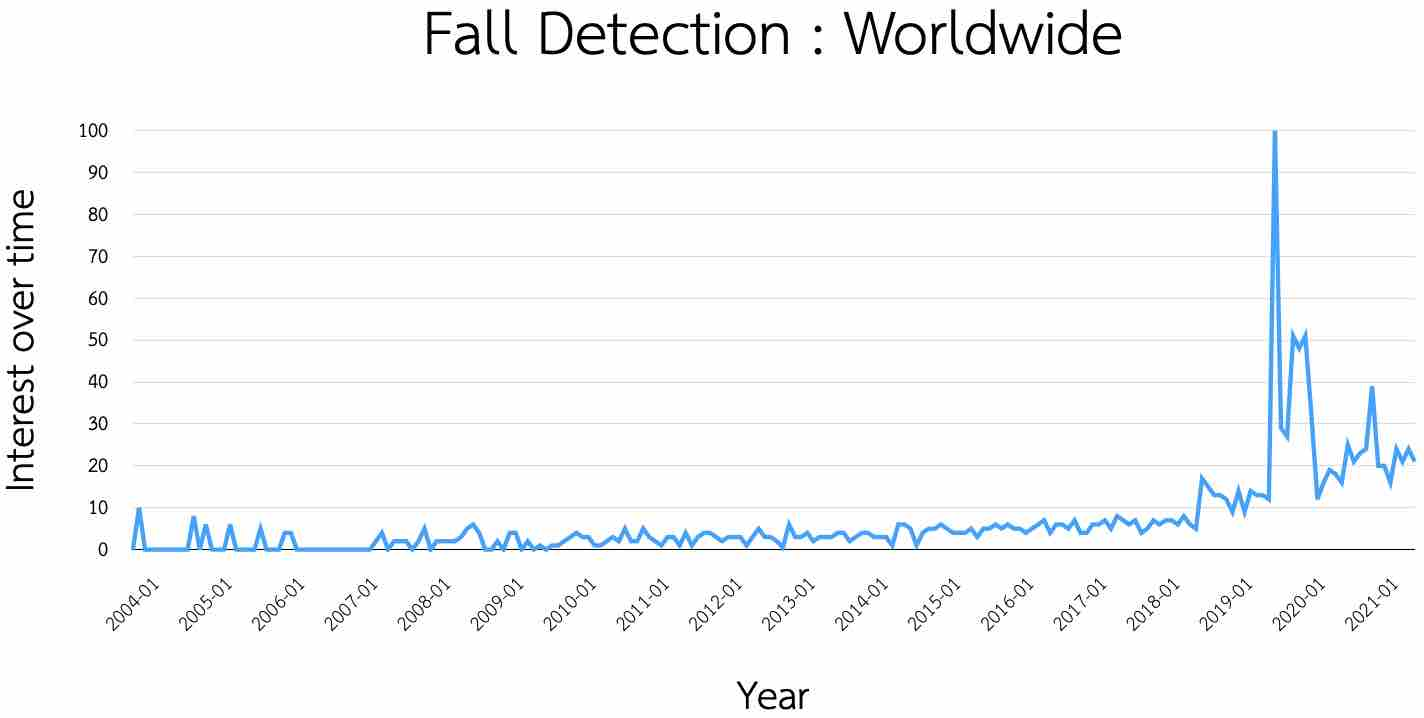
\includegraphics[width=\textwidth]{figures/fall_trend.jpg}
\end{figure}

\subsection{Fall detection by using vibration sensors}

Table \ref{tab:fall_review} shows the evolution of fall detection from floor vibration. Most researches use classifier models to detect fall events with training performed on simulated fall data that were not real falls. Furthermore, none of these researchers have deployed their system in real environments, so the real world performance of the models is not convincing. To overcome these weaknesses, I will apply anomaly detection to compensate for the rarity of events such as real falls and other or unseen patterns, and send alerts to the caretaker or an assistance who can take care of a victim who is alone as soon as possible.

\begin{table}[H]
  \begin{center}
    % \linespread{0.55}\selectfont\centering
    \caption[Summary of literature review for fall detection from floor vibration.]{Summary of literature review for fall detection from floor vibration. \\}\label{tab:fall_review}
    \begin{tabular}{m{0.13\linewidth} m{0.23\linewidth} m{0.18\linewidth} m{0.18\linewidth} m{0.2\linewidth} }
      \textbf{Authors}                                               & \textbf{Data Collection}                      & \textbf{Sensors}                                             & \textbf{Algorithms}                                                                & \textbf{Alarm}           \\
      \hline

      \shortciteA{Alwan_2003}                                        & Simulated by people.                          & N/A                                                          & Threshold                                                                          & N/A                      \\
      \hline
      \shortciteA{alwan_rajendran_kell_mack_dalal_wolfe_felder_2006} & Simulated by people and dummies.              & Piezoelectric                                                & Threshold                                                                          & Send messages to a pager \\
      \hline

      \shortciteA{litvak_zigel_gannot_2008}                          & Simulated by people and dummies.              & Microphone \newline Accelerometer                            & Gaussian model \newline Sequential forward floating selection (SFFS) \raggedright  & N/A                      \\
      \hline


      \shortciteA{davis_caicedo_langevin_hirth_2011}                 & Simulated by people.                          & N/A                                                          & Threshold                                                                          & N/A                      \\
      \hline

      \shortciteA{inproceedings}                                     & N/A                                           & Pyroelectric infeared (PIR) \newline Vibration sensor        & Support vector machine (SVM) \raggedright                                          & N/A                      \\
      \hline


      \shortciteA{shao_wang_song_ilyas_guo_chang_2020}               & Simulated by 3d-printed skeleton \raggedright & Accelerometer on smartphone                                  & K-nearest-neighbor (KNN)                                                           & N/A                      \\
      \hline

      \shortciteA{liu_jiang_su_benzoni_maxwell_2019}                 & Simulated by people and dummies.              & Seismic                                                      & A multi-features semi-supervised support vector machines (MFSS - SVM) \raggedright & N/A                      \\
      \hline

      \shortciteA{clemente_li_valero_song_2020}                      & N/A                                           & Seismic                                                      & One-class SVM                                                                      & N/A                      \\
      \hline

      \shortciteA{mukherjee2020multisense}                           & N/A                                           & Motion sensor \newline Heat sensor \newline Vibration sensor & Threshold                                                                          & N/A                      \\
      \hline
    \end{tabular}
  \end{center}
\end{table}

\section{Human Activity}

To create training data for anomaly detection in the home, it is important to cover all of the typical activities that people are expected to engage in in the home.


\citeauthor{schrader_2020} \citeyear{schrader_2020}  say there is no common definition or description of human activities because human activity is highly diverse. Nonetheless, the most fundamental activity in home is clearly walking, since a resident needs to move several inside the home to perform any other activities \cite{oukrich_2019}. There also are other general activities that every person does. I summarized activity catagories proposed in the literature on human activity in home in Table \ref{tab:human_activity}. Each paper in the table includes experiments on different activities of interest, and there are some common activities across most of the studies such as sitting, walking, standing and lying.

\begin{table}[H]
  \begin{center}
    \caption[Summary of literature review on human activity.]{\emph{Summary of literature review on human activity.}} \label{tab:human_activity}
    \begin{tabular}{m{0.2\textwidth} m{0.3\textwidth} m{0.2\textwidth} m{0.25\textwidth} }
      \textbf{Authors}                                                        & \textbf{Objective of study}                                       & \textbf{Related Sensors}                                                                             & \textbf{Identified Activities}                                                                                                                  \\
      \hline

      \shortciteA{roggen_2010} \raggedright                                   & Collect complex activity datasets in home \raggedright            & Microphone \newline Accelerometers \newline Gyroscope \newline Magnetometer \newline Inertial sensor & Sitting  \newline Walking \newline Standing \newline Lying                                                                                      \\
      \hline

      \cite{chen_xue_2015} \raggedright                                       & Classify human activity by single accelerometer \raggedright      & Accelerometer                                                                                        & Walking \newline Standing \newline Lying \newline Running \newline Rope jump \newline Vacuum cleaning \newline Downstairs \newline Upstairs     \\
      \hline

      \cite{reiss_stricker_2012} \raggedright                                 & Published a new public dataset for physical activity \raggedright & Gyroscope \newline Magnetometer                                                                      & Sitting \newline Step walking \newline Walking quickly \newline Falling \newline Jumping \newline Running \newline Downstairs \newline Upstairs \\
      \hline

      \shortciteA{ugolotti_sassi_mordonini_cagnoni_2011} \raggedright         & Detect and classify human activities \raggedright                 & Camera \newline Accelerometer                                                                        & Sitting \newline Walking \newline Standing \newline Lying \newline Get up \newline Fall \newline Rise                                           \\
      \hline

      \cite{abbate_avvenuti_bonatesta_cola_corsini_vecchio_2012} \raggedright & Detect fall events                                                & Accelerometer on smartphone                                                                          & Sitting \newline Walking \newline Lying \newline Running \newline Jumping \newline Hitting the sensor                                           \\
      \hline
    \end{tabular}
  \end{center}
\end{table}


\section{Floor Vibrations}

Movement in a building by residents during their normal activities causes floor vibration. This vibration is normally vertical \cite{steelconstruction_2016}. Floor vibrations are generated by dynamic loads caused directly by people (e.g. walking, dancing, jumping) or machinery, or they may be generated indirectly by the external environment (e.g. traffic). Theoretically, vibrations are cyclic motions with two significant attributes, frequency and amplitude. In practice, floor vibrations are quite complex dynamic systems with unlimited vibrational modes. \citeauthor{ljunggren2006floor} \citeyear{ljunggren2006floor} summarises the parameter that influence the dynamic system of a floor:
\begin{itemize}
  \item Stiffness ($k$): Stiffness controls the springiness of the floor. Higher stiffness can decreases the vibrational amplitude occurring due to a force.
  \item Damping ($\zeta$): This factor depends on the material making up the surface. It is extremely difficult to obtain an exact damping value.
  \item Mass ($M$): Higher mass surfaces have reduced vibrational amplitudes. Lower mass is desirable if we want to observe vibrations. However, when the mass is too little, the resulting strong vibrations may disturb residents.
  \item Fundamental frequency: Floor vibrations are assumed to be occur mainly at a natural frequency, which depends on the stiffness and the mass. Higher frequencies are usually less annoying to residents than lower frequencies.
\end{itemize}

The complexities of the dynamic system can be modeled as a series of simple mass and spring models with a single degree of freedom \cite{p_gavin_2015}. The characteristics of a vibration model are illustrated in Figure \ref{fig:s_degree}.

\begin{figure}[H]
  \centering
  \caption[Single degree of freedom system mass-spring model for floor vibration.]{\emph{Single degree of freedom system mass-spring model for floor vibration. \\ Reprinted from \citeauthor{steelconstruction_2016} \citeyear{steelconstruction_2016}.}  }\label{fig:s_degree}
  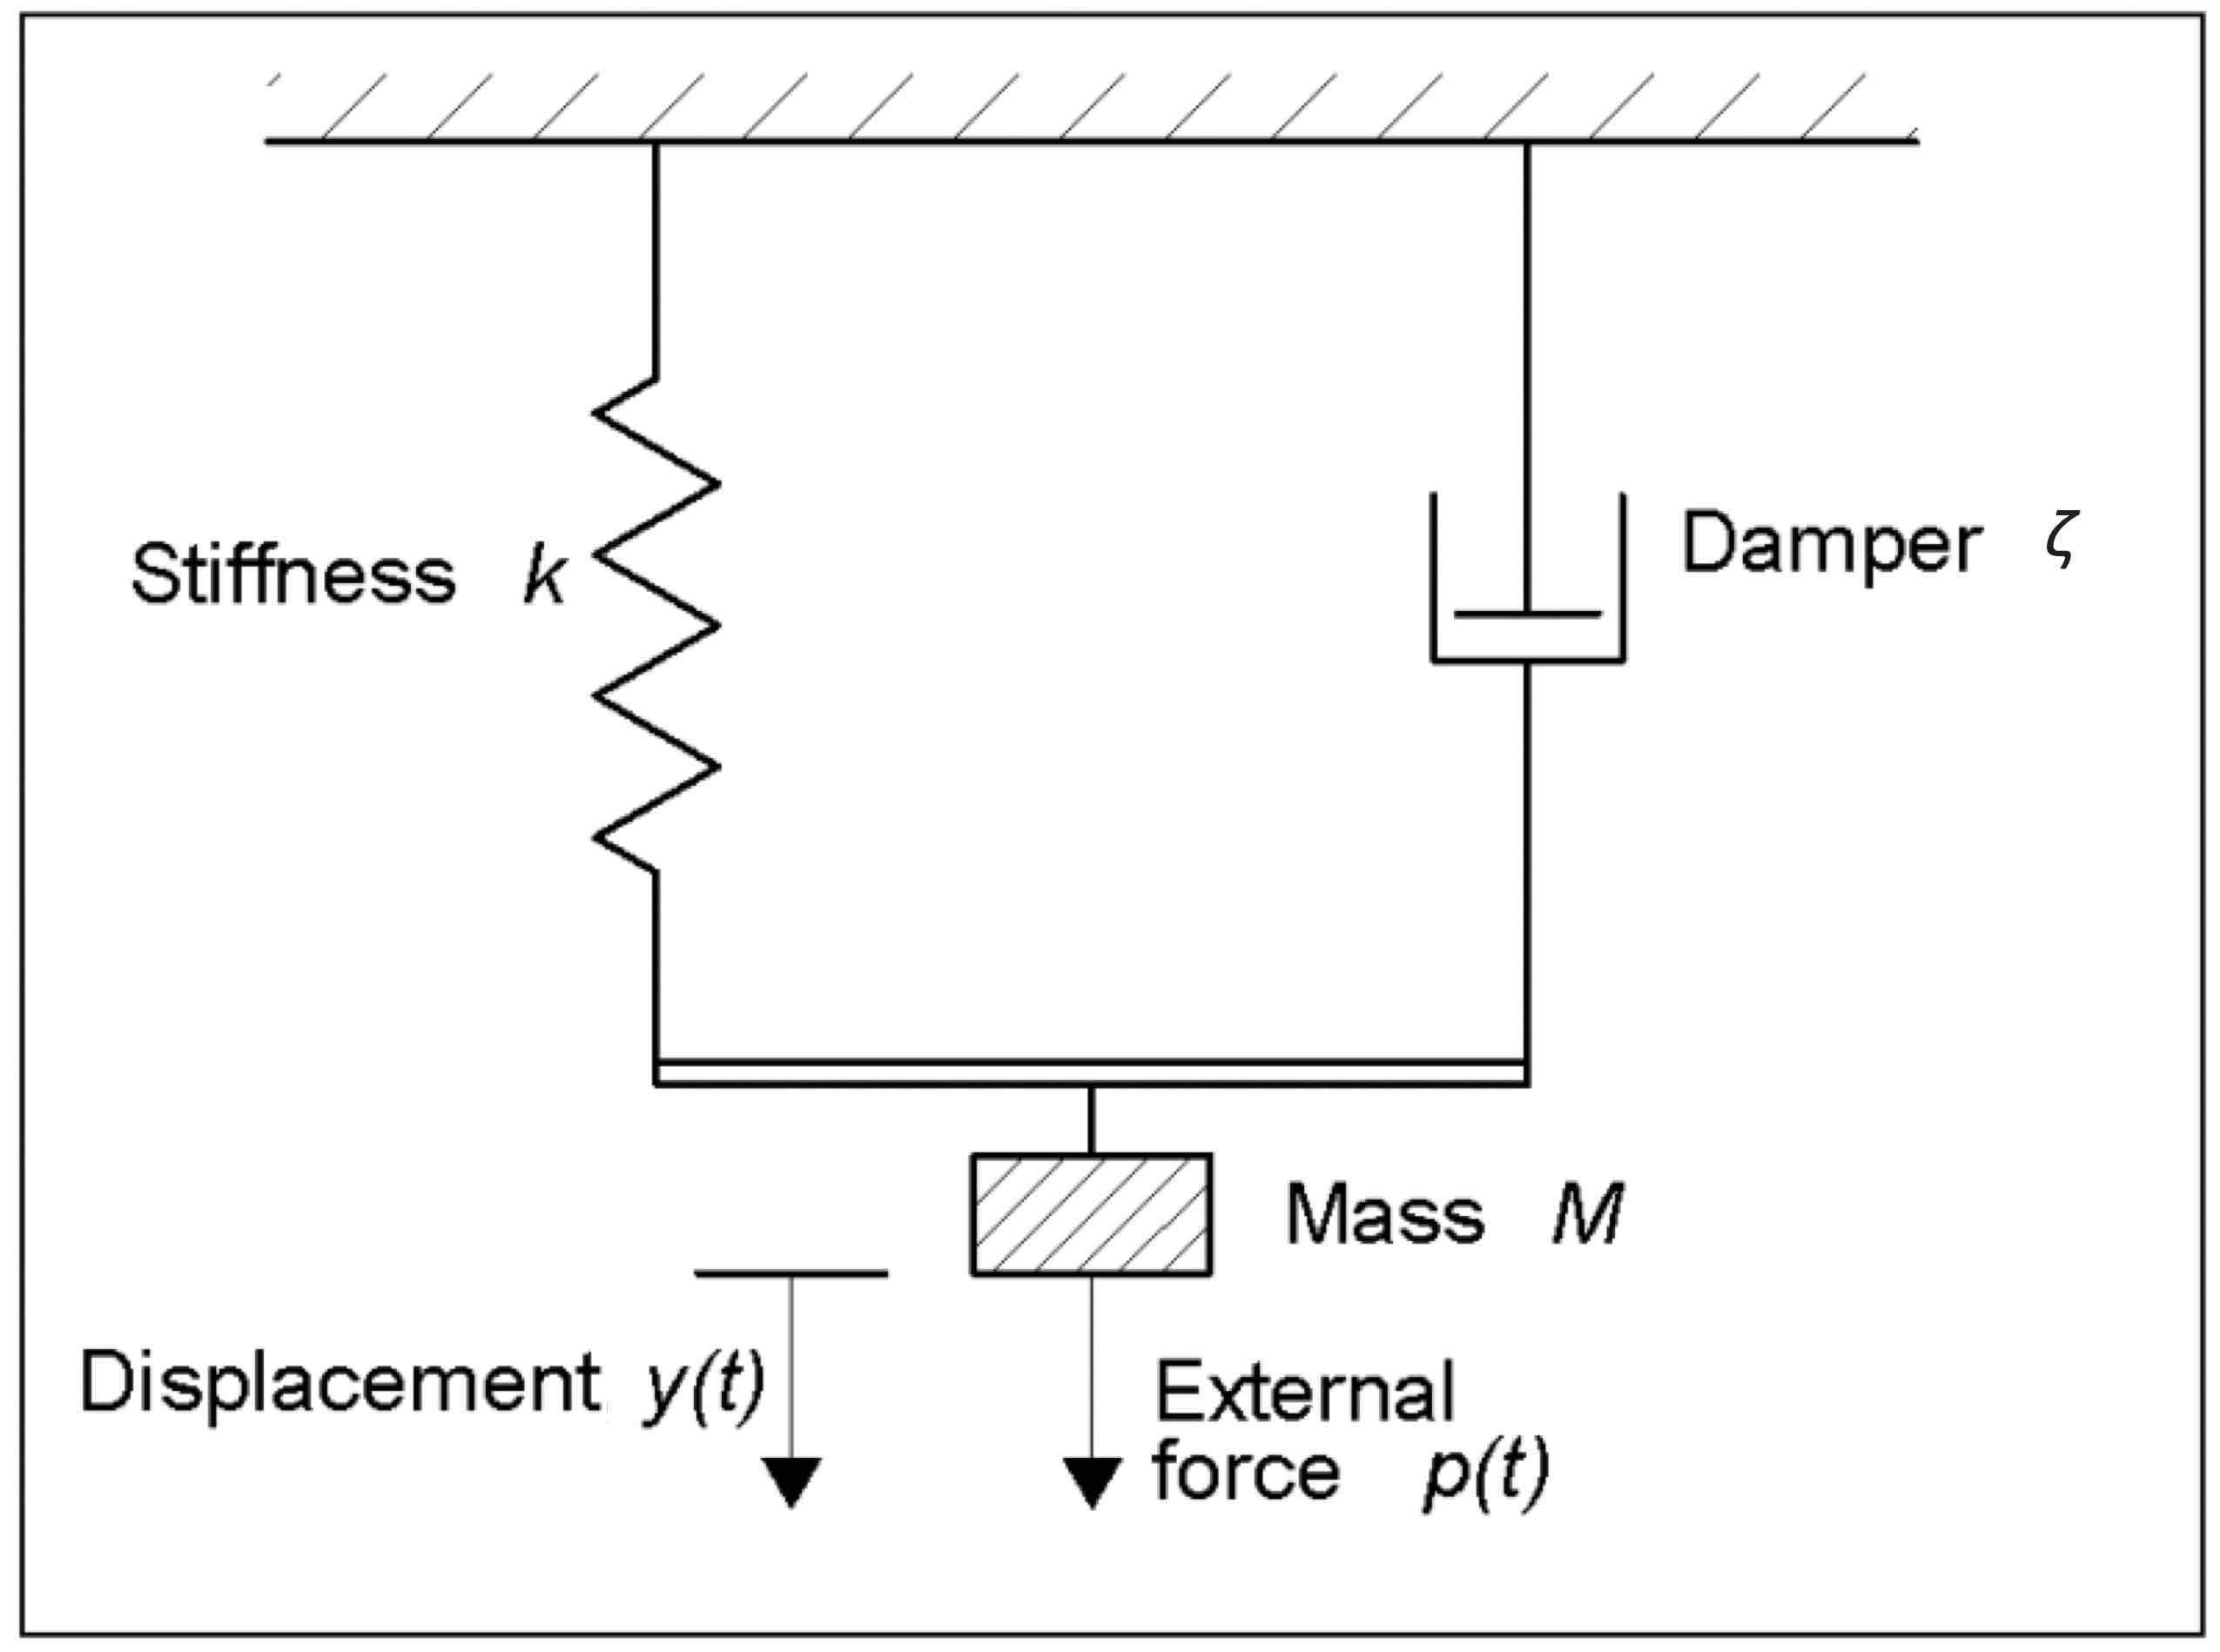
\includegraphics[scale = 0.13]{figures/single_degree.jpg}
\end{figure}

\section{Time Series}

A time series is a sequence of measurements of a particular random variable at specific sequence of discrete points in time. Generally, the data should be sampled at a constant interval expresssed in as seconds, minutes, hours, days, months, and/or years. In time series analysis, we would generally like to predict a target variable at particular time lags given a window of previous measurements. This is unusual in that in ordinary supervised classification or regression, the target at time $t$ is not used as a feature at a later time, but in time series analysis, this is often the case.


There are many diverse techniques for analyzing sequential data. The simplest techniques are a special case of regression analysis in which we want to capture four different elements as following \cite{dash_2020}:
\begin{itemize}
  \item Seasonal variations: repeating shape or appearance occuring during a specific period such as daily, weekly, monthly, or seasonally.
  \item Trend: possible trends are upwards, downwards, or constantard can be linear or nonlinear.
  \item Cyclical variations: movement that follows a specific cyclic period such as business cycles. Cyclical variations are similar to seasonal variations but have different underlying cases specific to the particular problem.
  \item Random variations: the variation remaining after the first three types of predictable variation are accounted for.
\end{itemize}

\subsection{Autoregressive (AR)}

Autoregressive models, the simplest time series models, which are used for predict or forecasting proposes, operate under the assumption that each new value depends on some or all of the the past values. The generative model for a linear of autoregressive process is shown below:

\hfil $Y_t = \varphi_1Y_{t-1} + \cdots + \varphi_pY_{t-p} + \epsilon_t $ \par

where $\epsilon \sim N(0, \sigma^2)$. p is the order of the model, which we write as AR(p). For example, AR(1) means the observation at time $t$ depends only on the observation at time $t-1$ plus noise, whereas. AR(2) means $y_t$ depends on the previous two values as well as a noise sample.

\subsection{Time series classification}

Over the last two decades, one of the most challenging problems in data mining is a classification of time series \cite{ismail_fawaz_forestier_weber_idoumghar_muller_2019}. Several methods have emerged for time series classification. The naive algorithm is Euclidean maching, which is not normally effective without some modification. On the other hand, dynamic time warping (DTW) is an outstanding baseline, and the current state of the art would in the most cases be represented by deep learning classifiers. Dynamic time warping is based on an alignment cost computed between two data sequences that can be stretched or shrunk to accommodate variations along the time axis \cite{meinard_2007, toyoda_sakurai_2012}. Consider two sequences, $X = (x_1, x_2, ..., x_n)$ of length $n$ and $Y = (y_1, y_2, ..., y_m)$ of length $m$. The DTW distance $D(X,Y)$ is defined as:

\hfil $ D(X, Y) = D(m, n)$ \par
\hfil $ D(i,j) = (x_i - y_j)^2$ + $\min$ $\begin{cases} $D(i-1, j)$ \\ $D(i-1, j-1)$ \\$D(i, j-1)$ \end{cases}$  \par
where $D(0, 0) = 0$, $D(i, 0) = D(j, 0) = \infty$, $i = (1, 2, ..., n)$ and $j = (1,2, ...,m)$.


\begin{figure}[H]
  \centering
  \caption[Euclidean maching versus DTW matching.]{\emph{Euclidean maching versus DTW matching. \\
      Reprinted from Dynamic time warping \cite{dtw_2021}.}}\label{fig:DTW}
  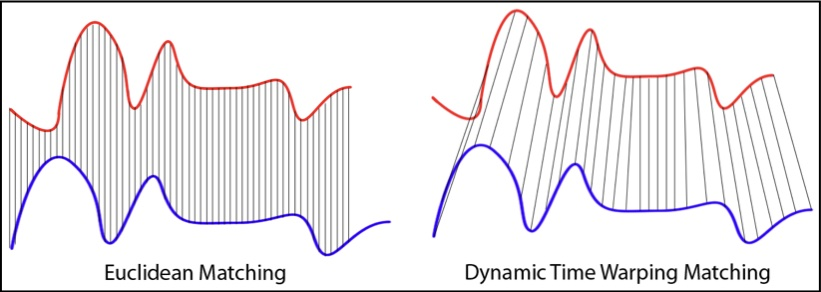
\includegraphics[scale = 0.5]{figures/DTW.jpg}
\end{figure}



DTW can be used not only for pattern matching or classification, but also for anomaly detection. If the distance between a new signal and each signal in a gallery of historical signals is higher than a set threshold, we can conclude the new signal is an anomaly. The main weaknesses of dynamic time warping is its long processing time. Some more effective learning-based approaches are explained in the following sections.

\subsection{Convolutional Neural Network (CNN)}

A Convolutional neural network is a deep learning model whose input can be an image, video, spatial data, or any multidimensional tensor with locality. One-dimensional CNNs can be used on general data types including text tokens and other types of time series data. CNNs capture spatial and temporal dependencies in a dataset through convolutional filters. A convolution kernel is local linear filter that is slid over the imput tensor along one or more dimensions to obtain a feature map as shown in Figure \ref{fig:CNN}. The general method for temporal CNN layer with a nonlinear activation function is

\hfil $C_t = f(W \cdot X_{t-l/2 \to t+l/2} + b) | \forall t \in [1, T], $ \par \

\begin{figure}[H]
  \centering
  \caption[Convolving on univariate input time series.]{\emph{Convolving on univariate input time series. \\
      Reprinted from \citeauthor{ismail_fawaz_forestier_weber_idoumghar_muller_2019} \citeyear{ismail_fawaz_forestier_weber_idoumghar_muller_2019}.}}\label{fig:CNN}
  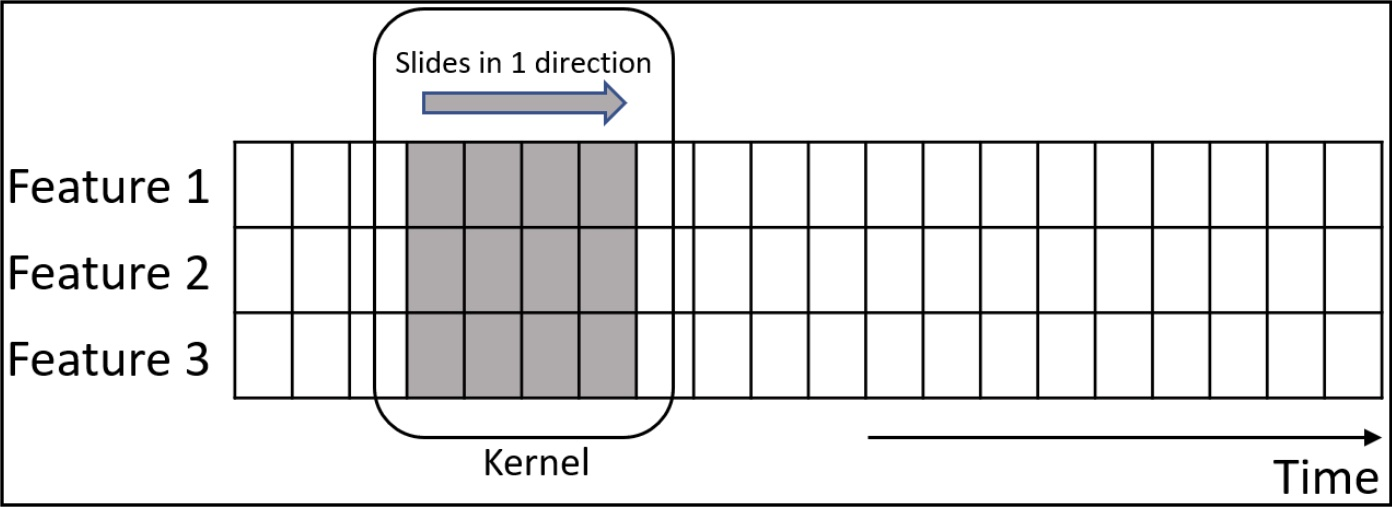
\includegraphics[scale = 0.3]{figures/CNN.jpg}
\end{figure}


where $C_t$ is the result of the convolution operation at time $t$ on time series $X$ of length $T$ with a filter $W$ of length $l$, a bias parameter $b$, and a final non-linear function $f$. It can be noticed that the same filter values $W$ and bias $b$ are used at every timestep, a very significant and useful property called weight sharing. When a series of convolutions are completed, the resulting feature maps would typically be fed though fully-connected layer as in the simple neural network architecture shown in Figure \ref{fig:CNN_ts}.

\begin{figure}[H]
  \centering
  \caption[Typical temporal convolutional neural network architecture.]{\emph{Typical temporal convolutional neural network architecture.  \\
      Reprinted from \citeauthor{ismail_fawaz_forestier_weber_idoumghar_muller_2019} \citeyear{ismail_fawaz_forestier_weber_idoumghar_muller_2019}.}}\label{fig:CNN_ts}
  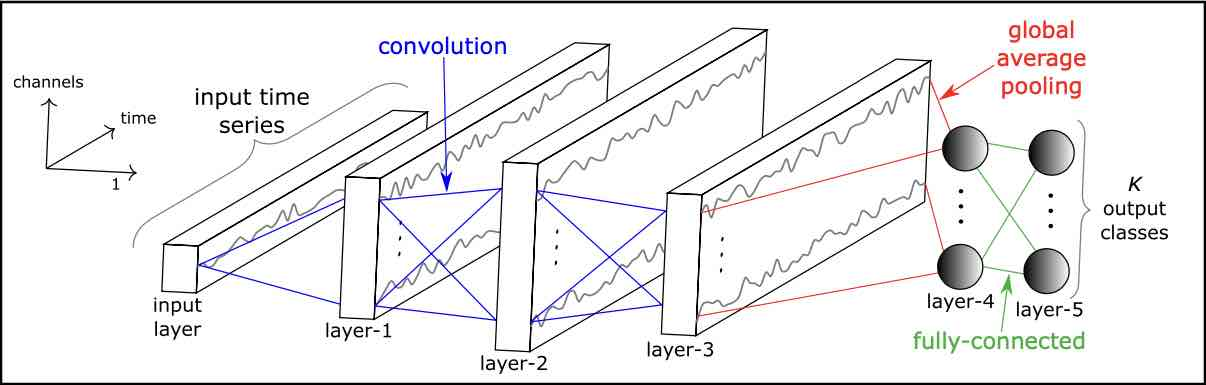
\includegraphics[scale = 0.3]{figures/CNN_ts.jpg}
\end{figure}



\section{Autoencoders}

An autoencoder is a neural network able to compress data similar to what it was trained on. Autoencoders do not require labeled data for training since they utilize unsupervised learning. We just feed the raw input into the model. Figure \ref{fig:ae} illustrates the intuition of how an autoencoder works.


Besides compression, an autoencoder can be used for denoising by training the autoencoder to reproduce an original noiseless input given a noisy input. This allows the autoencoder to be flexible in the presence of white noise capturing only useful patterns in the data \cite{vincent10a}.

\begin{figure}[H]
  \centering
  \caption[An autocoder workflow.]{\emph{An autocoder workflow. \\
      Reprinted from \citeauthor{chollet_2016} \citeyear{chollet_2016}.}}\label{fig:ae}
  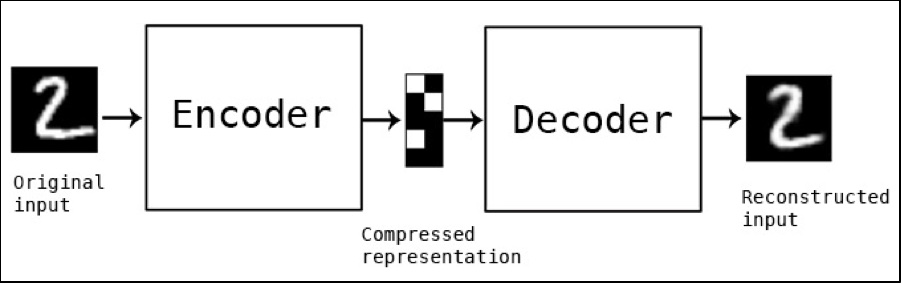
\includegraphics[scale = 0.5]{figures/ae.jpg}
\end{figure}


An autoencoder has three main components \cite{badr_2019}: the encoder, the code or bottleneck, and the decoder, as shown in Figure \ref{fig:ae_architecture}.
\begin{itemize}
  \item Encoder: Learns how to reduce input dimensionality, compressing the input data into an encoded representation.
  \item Bottleneck: The layer that contains the compressed representation of the input data. This code space is also called the latent space.
  \item Decoder: Learns how to reconstruct as closely as possible the input pattern from the encoded representation.
\end{itemize}

\begin{figure}[H]
  \centering
  \caption[The autoencoder architecture.]{\emph{The autoencoder architecture. \\
      Reprinted from \citeauthor{pedamkar_2019} \citeyear{pedamkar_2019}.}}\label{fig:ae_architecture}
  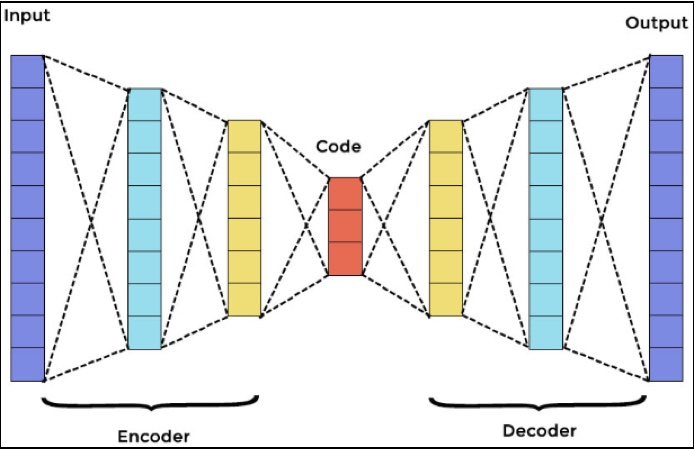
\includegraphics[scale = 0.5]{figures/ae_architecture.jpg}
\end{figure}


The indirect benefits of this model is that it can be used for dimensionality reduction \cite{rajan_2021}. The bottleneck has the fewest units of any layer. An example of the kinds of compression an autoencoder can achieve is shown in Figure \ref{fig:ae_f_reduction}. This model reduces the three dimensional input to two dimensions.


\begin{figure}[H]
  \centering
  \caption[Visualization of dimensionality reduction using autoencoders.]{\emph{Visualization of dimensionality reduction using autoencoders. \\
      Reprinted from Johns Hopkins University \citeyear{johns_hopkins_university_2015}.}}\label{fig:ae_f_reduction}
  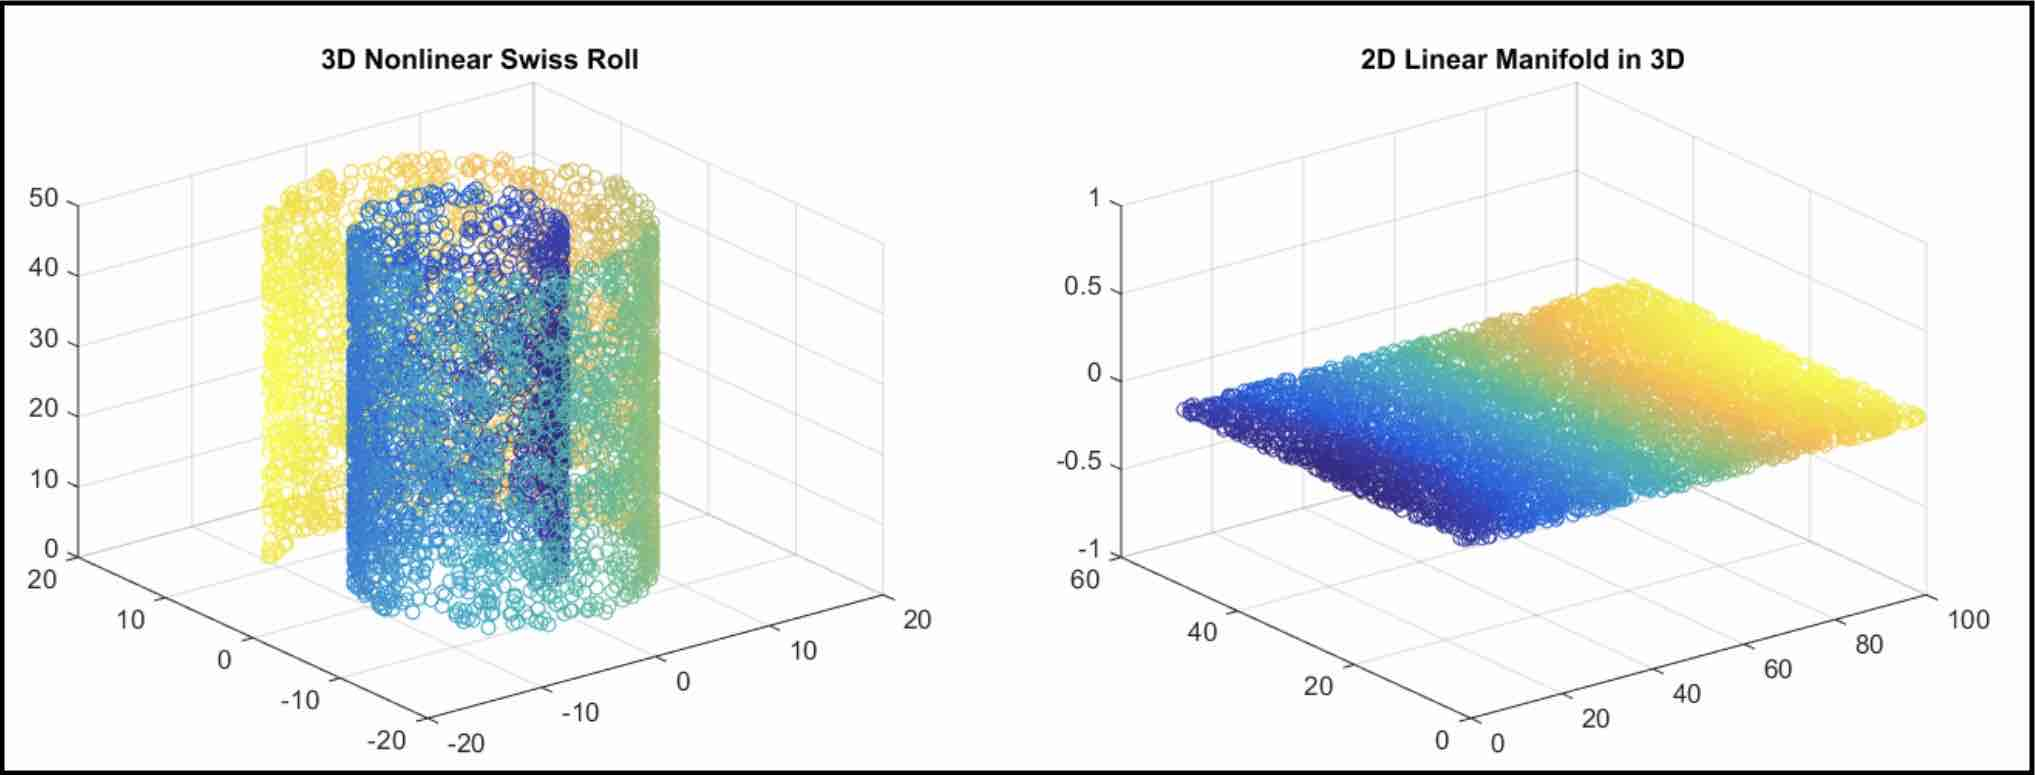
\includegraphics[scale = 0.2]{figures/ae_f_reduction.jpg}
\end{figure}


Besides compression, an autoencoder can be used for denoising by training the autoencoder to reproduce an original noiseless input given a noisy input, as shown in Figure \ref{fig:ae_2}. This is because the optimizer encodes the inputs it was trained on as much as possible. \citeauthor{vincent_larochelle_bengio_manzagol_2008} \citeyear{vincent_larochelle_bengio_manzagol_2008} found that the robustness of the code at the bottleneck was improved by adding noise to the original input. This allows the autoencoder to be flexible in the presence of white noise capturing only useful patterns in the data \cite{vincent10a}.


\begin{figure}[H]
  \centering
  \caption[An autoencoder trained on ``clean" images can correct noisy input.]{\emph{An autoencoder trained on ``clean'' images can correct noisy input. \\
      Reprinted from \citeauthor{rosebrock_2020} \citeyear{rosebrock_2020}.}}\label{fig:ae_2}
  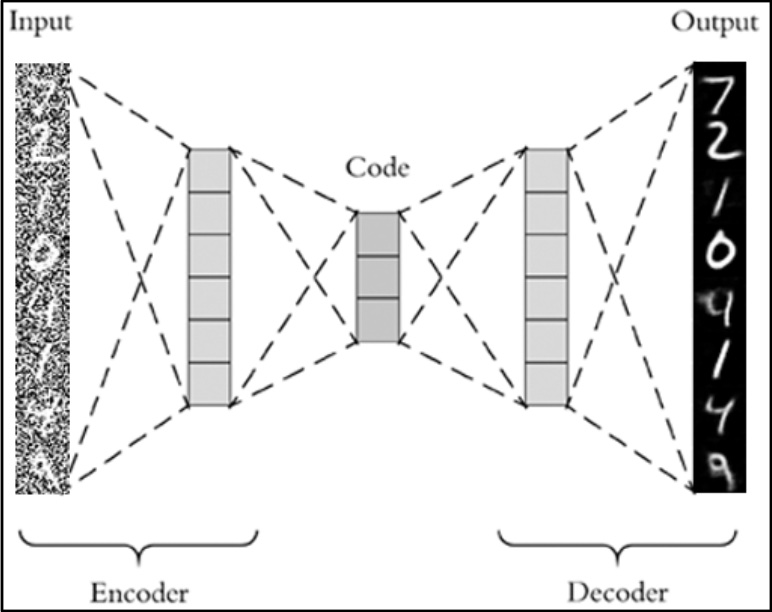
\includegraphics[scale = 0.4]{figures/ae_2.jpg}
\end{figure}


Beside the simple feedforward layers described previously, autoencoder can be combined with long short term memory networks (LSTMs) or convolutional neural networks (CNNs) depending on the type of input. In my thesis, the input, vibration from human activities, is a sequential time series. Therefore, an combination of autoencoder with LSTM networks may be suitable for my purpose.

\subsection{Autoencoders for Anomaly Detection}


Autoencoders are extremely useful as methods of typicality. Consider a person who does the same things every day. Suppose that one day, an unusual event occurs. An autoencoder trained on the usual daily activities will map the new situation to something similar in the training, as shown in Figure \ref{fig:ae_detection}. The reconstruction error in abnormal causes should be high. A model trained on one type of data (the normal activities) will fail when facing abnormal data it has never seen before. The simple autoencoder-based anomaly detection algorithm is shown in Algorithm \ref{al:anomaly_detection_algorithm}.

\begin{figure}[H]
  \centering
  \caption[An autoencoder capable of detecting anomalous events in time series.]{\emph{An autoencoder capable of detecting anomalous events in time series. \\ Reprinted from \citeauthor{pavithrasv_2020} \citeyear{pavithrasv_2020}.}}\label{fig:ae_detection}
  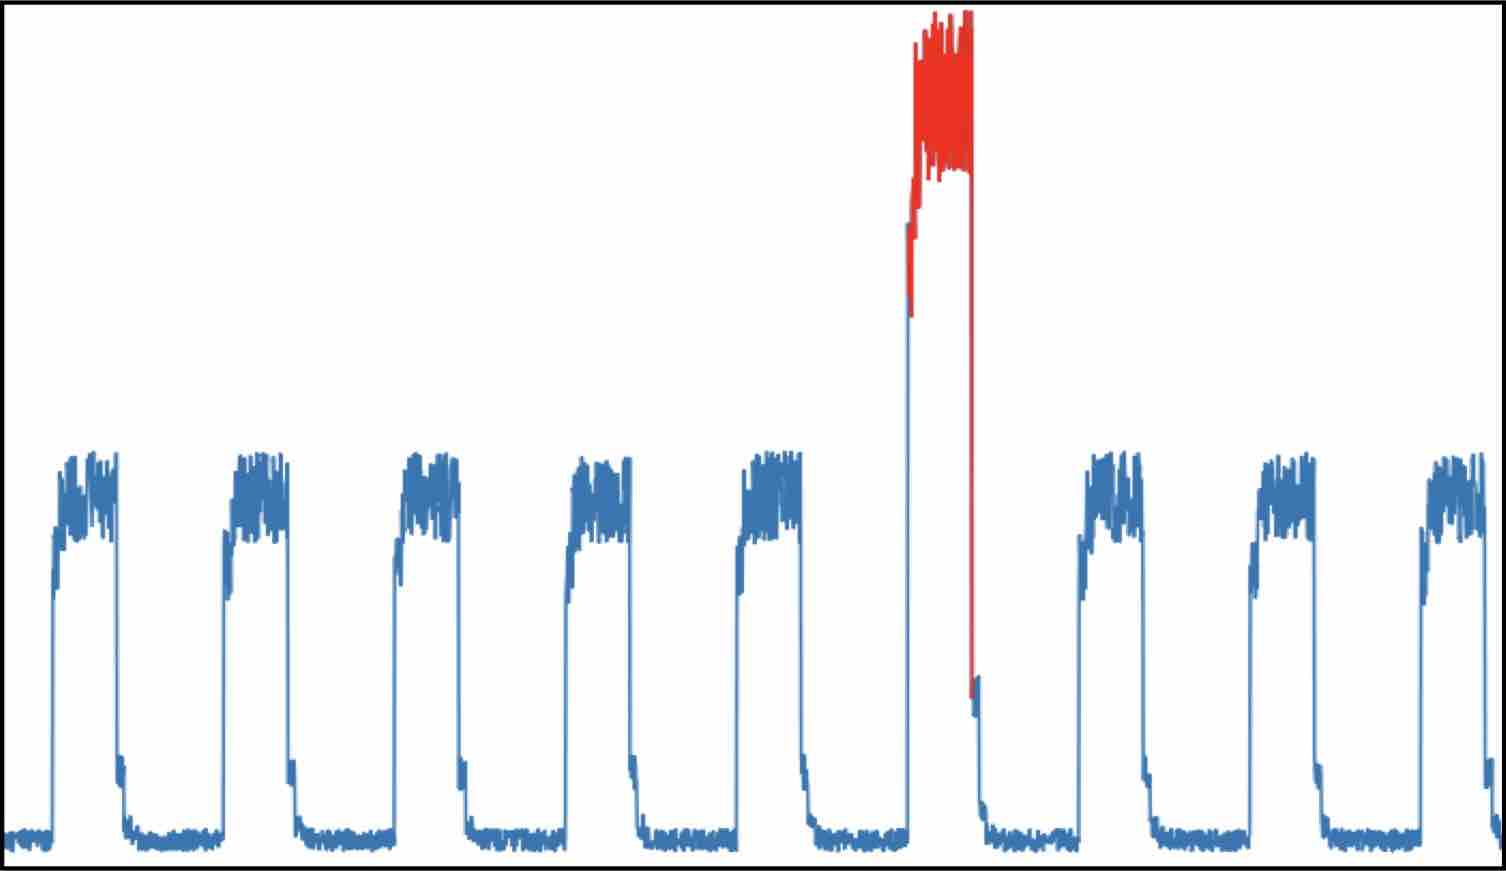
\includegraphics[scale = 0.2]{figures/ae_detection.jpg}
\end{figure}

\renewcommand{\algorithmicrequire}{\textbf{Input:}}
\renewcommand{\algorithmicensure}{\textbf{Output:}}
\renewcommand{\algorithmicforall}{\textbf{for each}}

\begin{algorithm}[H]
  \caption{Autoencoder-based anomaly detection }
  \label{al:anomaly_detection_algorithm}
  \begin{algorithmic}
    \REQUIRE Normal dataset: $X^{(i)} (i = 1,..., m)$, abnormal dataset: $x^{(j)}$ $(j = 1, ..., n)$, threshold: $\alpha$
    \ENSURE Reconstruct data: $\hat{X}$
    \STATE Reconstruction error: $\| X - \hat{X} \|$
    \STATE Train an autoencoder using the normal dataset X $\rightarrow$ $L^* = \underset{L} {\operatorname{argmin}} \sum_{i=1}^m \| {X}^{(i)} - \hat X^{(i)} \| ^ 2$
    \STATE Testing an autoencoder:
    \STATE \textbf{for} j = 1 to $n$ \textbf{do}:
    \STATE \indent \textbf{if} reconstruction error $<$ $\alpha$:
    \STATE \indent \indent $x^{(j)}$ is a nomal.
    \STATE \indent \textbf{else}:
    \STATE \indent \indent $x^{(j)}$ is an anomaly.
  \end{algorithmic}
\end{algorithm}

\subsection{Variational Autoencoder}

The variational autoencoder (VAE) is a generative model like the ordinary autoencoder, it encodes and decodes data in the training set, but it also attempts to model the probability density over the input space of the examples emitted by the data source, by transforming, e.g., Gaussian distributied latent vectors to elements of the input space. For example, if model is trained with traffic images, the decoder, when passed a sample from the code space, would have a high probability of emitting vehicle images object related to traffic. Other data would have a low probability of being emitted. By sampling in the latent space reconstructing, the variational autoencoder can also generate new examples that look similar to those from the original dataset \cite{roger_2021}. In the other words, a variational autoencoder is an encoder which is trained to be regularized at the bottomneck in order to guarantee that latent space is a good source for the generative process \cite{rocca_2020}. The architecture of a variational autoencoder is illustrated in Figure \ref{fig:VAE}. The latent space of a variational autoencoder is easy to sample from.

\begin{figure}[H]
  \centering
  \caption[Architecture of a variational autoencoder.]{\emph{Architecture of a variational autoencoder. \\
      Reprinted from \citeauthor{weng_2018} \citeyear{weng_2018}.}}\label{fig:VAE}
  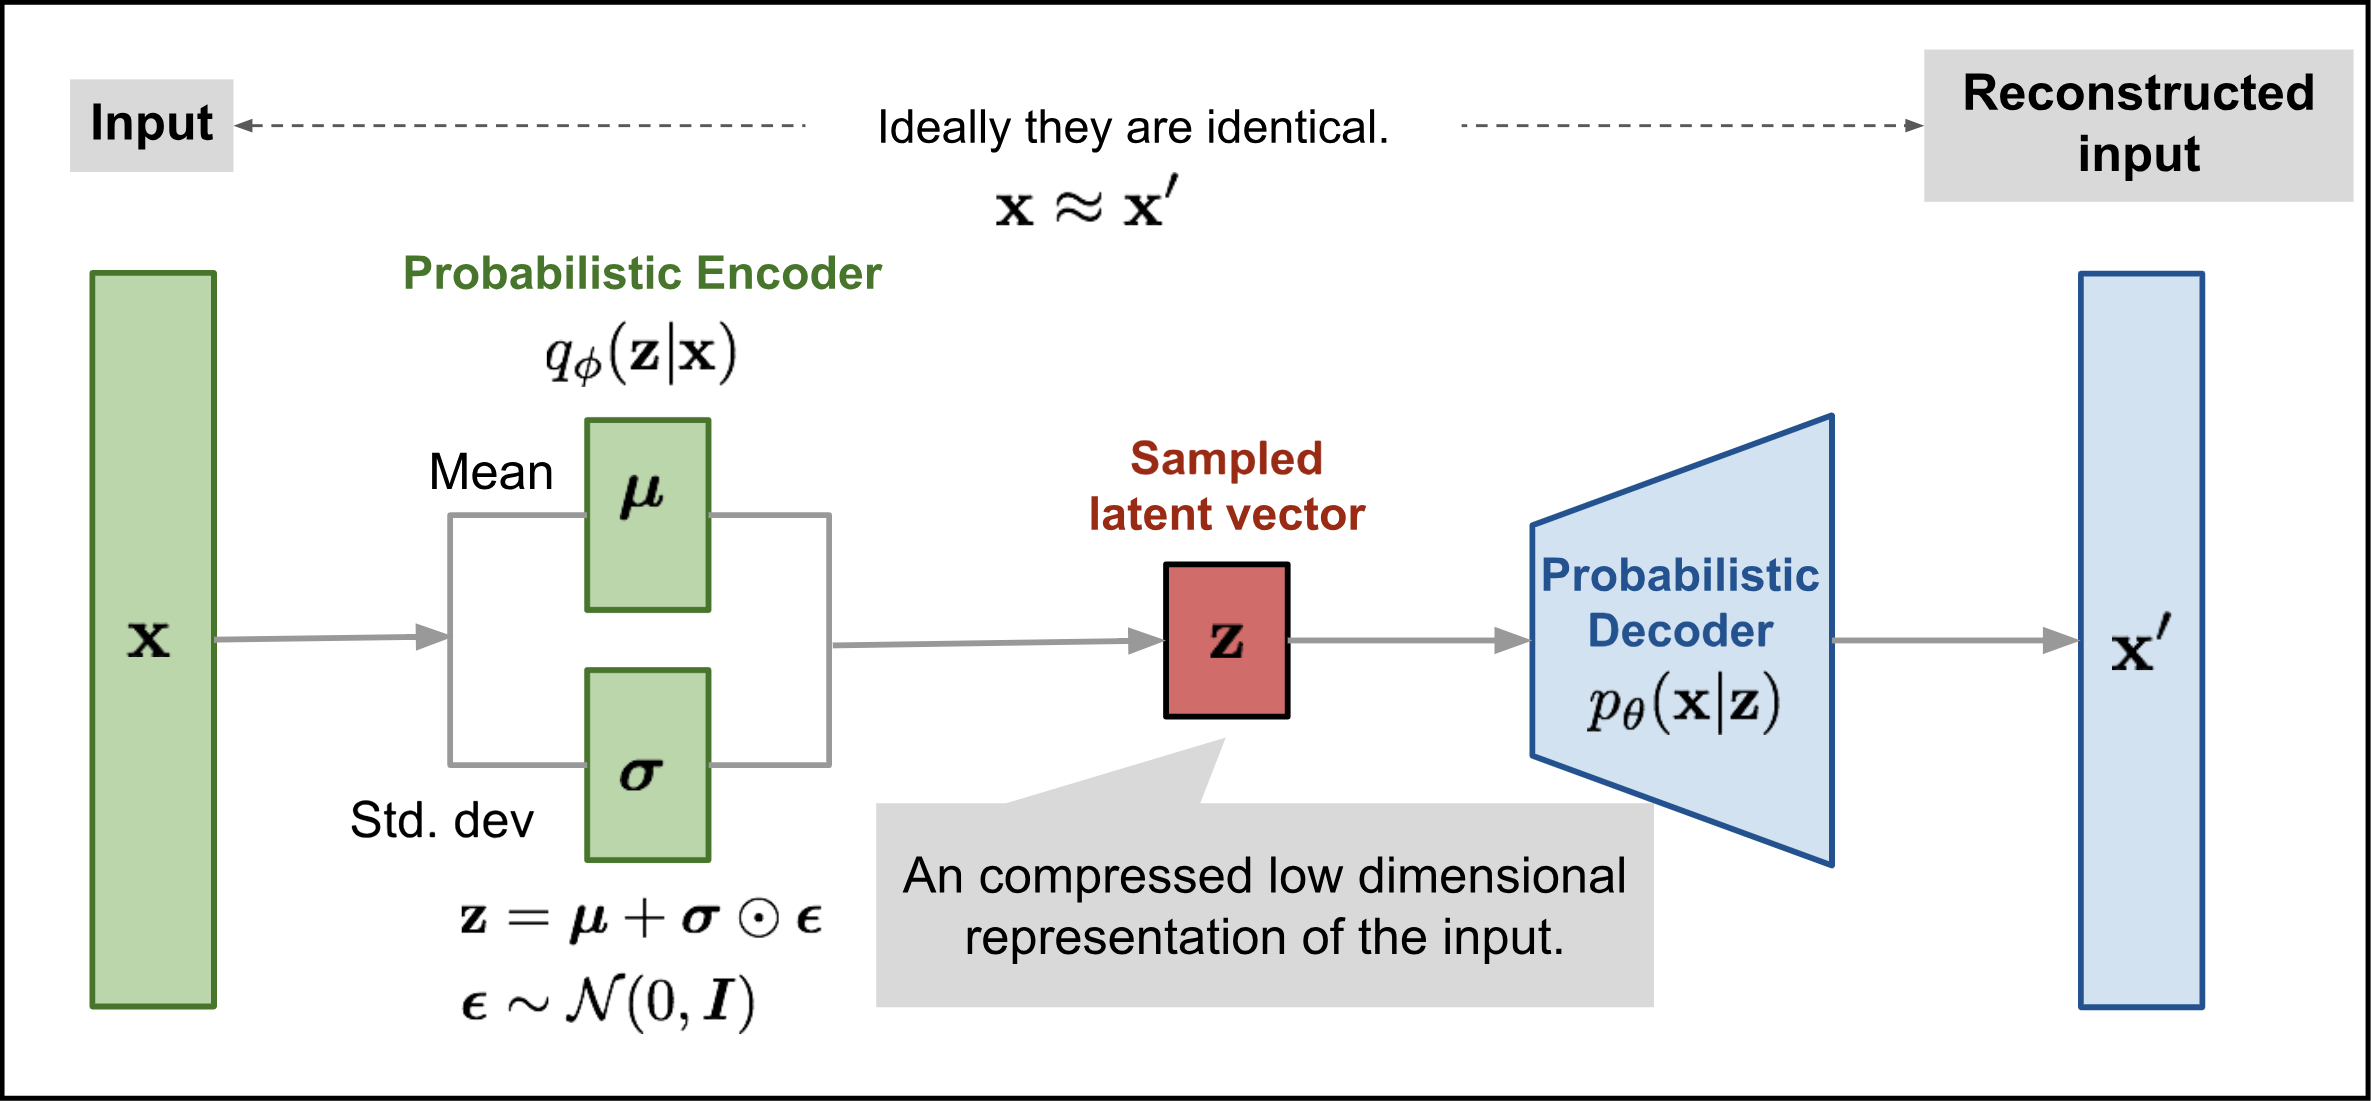
\includegraphics[scale = 0.15]{figures/VAE.jpg}
\end{figure}


The principles mentioned above do not mean that a variational autoencoder always has better performance than general autoencoders in anomaly detection tasks \cite{agmon_2021}, since the objective of the variational autoencoder is as a generative model for new data.

\section{Generative Adversarial Networks (GANs)}

The generative adversarial networks was first introduced in the paper ``Generative Adversarial Nets'' \cite{goodfellow_pouget_abadie_mirza_xu_warde_farley_ozair_courville_bengio_2014}. GANs consist of two networks, the generator and discriminator. The generators try to fool the discrimitor by creating virtual image. The discriminator try to distinguish different between real images and virtual images that were generated by the generator. Figure \ref{fig:GAN} illustrates the intuition of GAN. The both networks always fight together what is called adversarial training. The important idea is that we want the two networks learn from each other. During training, the generator can improve its performance to create images that look similar to the real images as well as possible. The discriminator also impove to distinguish. When training process reaches equilibrium, the discriminator is no longer able to distinguish the real from the fake, as shown in Figure \ref{fig:GAN_training}. Thus, if the discriminator is well trained and the generator can produce realistic-looking images that fool the discriminator, we have a good generator creating an image that looks like a training set.

\begin{figure}[H]
  \centering
  \caption[Representation of GAN as a generator and a discriminator.]{\emph{Representation of GAN as a generator and a discriminator. \\
      Reprinted from \citeauthor{ai_research_innovationhub_2020} \citeyear{ai_research_innovationhub_2020}.}}\label{fig:GAN}
  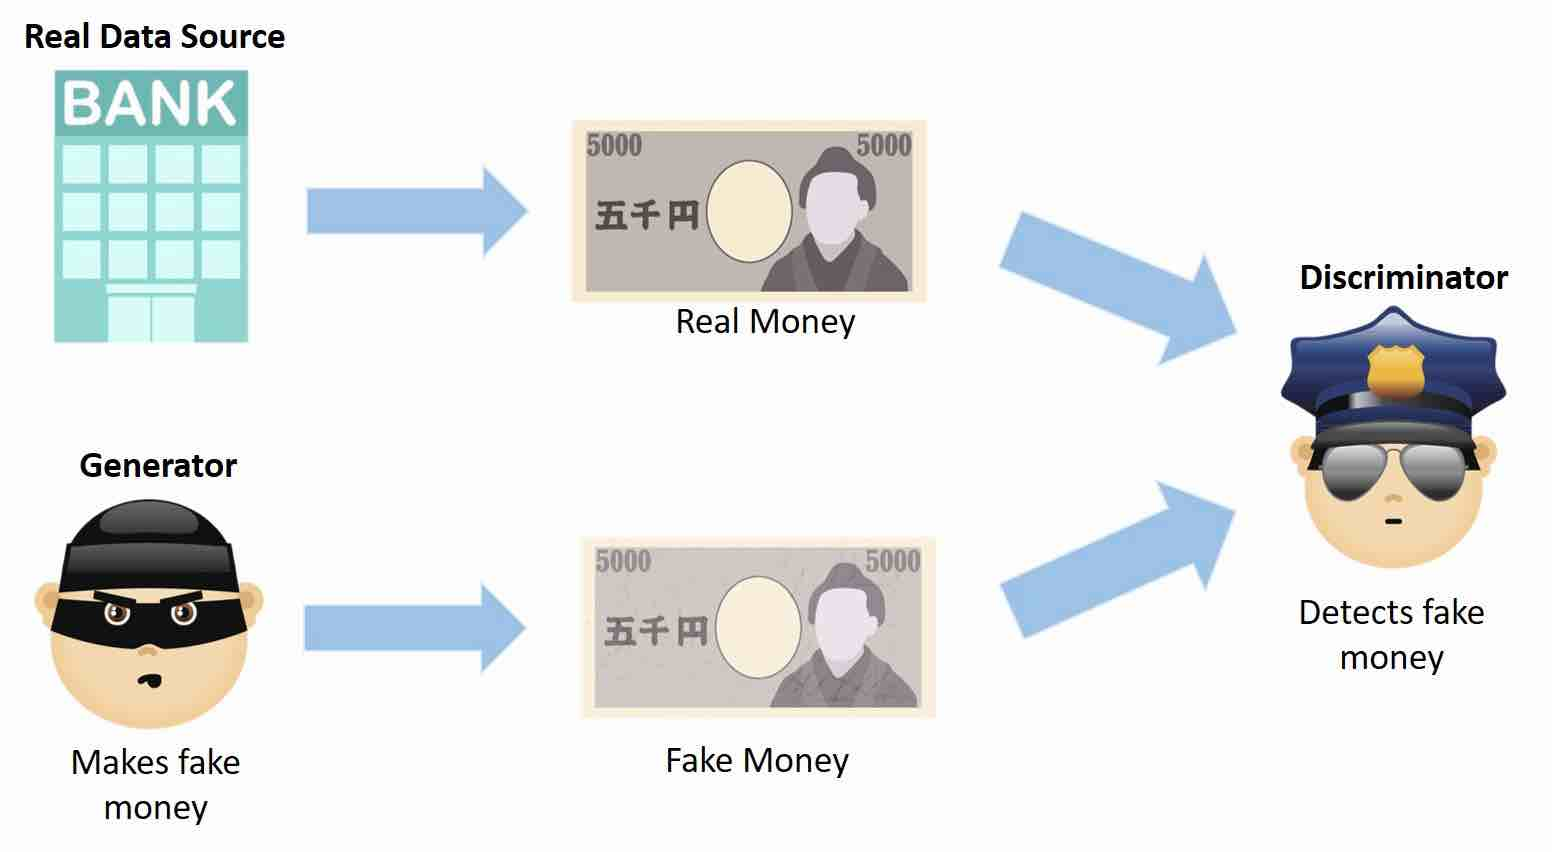
\includegraphics[scale = 0.3]{figures/GANs.jpg}
\end{figure}

\begin{figure}[H]
  \centering
  \caption[Training of the generator and discriminator.]{\emph{Training of the generator and discriminator. \\
      Reprinted from \citeauthor{tensorflow_2021} \citeyear{tensorflow_2021}.}}\label{fig:GAN_training}
  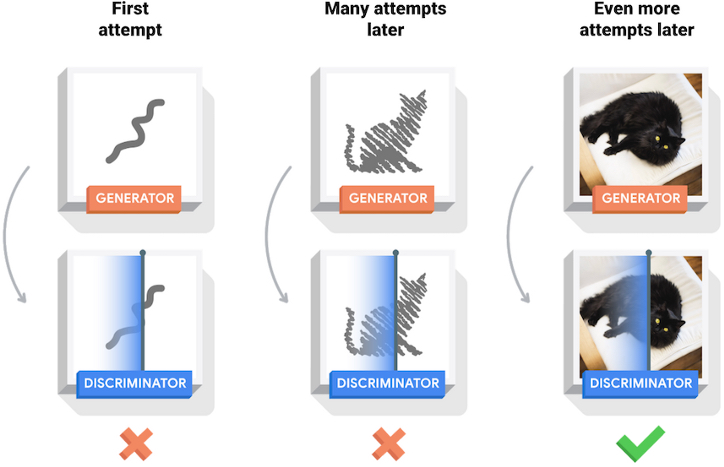
\includegraphics[scale = 0.5]{figures/GAN_2.jpg}
\end{figure}

\subsection{Generative Adversarial Networks for Anomaly Detection}

Anomaly detection by using GANs is possible. \shortciteA{schlegl2017unsupervised} \citeyear{schlegl2017unsupervised} firstly proposed AnoGAN, a deep convolutional generative adversarial network, to detect abnormal image. AnoGAN's architecture is based on standard GAN. AnoGAN is trained only on normal samples, which can lead the generator learning to generate normal samples. When an anomalous or unseen image is fed though the model, the difference between the input and the reconstructed images will be highlight the anomaly area, as shown in Figure \ref{fig:GAN_anomaly}.

\begin{figure}[H]
  \centering
  \caption[Anomaly detection using AnoGAN.]{\emph{Anomaly detection using AnoGAN. \\
      Reprinted from \citeauthor{schlegl2017unsupervised} \citeyear{schlegl2017unsupervised}.}}\label{fig:GAN_anomaly}
  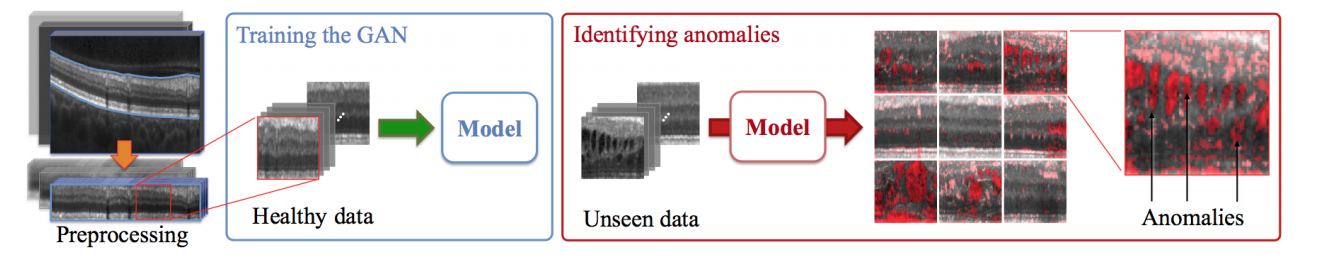
\includegraphics[scale = 0.35]{figures/GAN_anomaly.jpg}
\end{figure}



\section{Recurrent Neural Networks (RNNs)}

The main idea of recurrent neural networks (RNNs) is to process sequential data such as videos (sequences of images) or text (sequences of words). For example, when we read a book, we observe a sequence of tokens (words) as we read from left to right. To understand what the sentence is about, we observe each token in the sequence, and mix it with the meaning of the words we previously read. A RNN uses the same principle, by modifying simple feedforward neural networks so that the previous state can be combined with new inputs in a sequential time series \cite{donges_2019}. A key attribute of RNNs is their ability to retain the results of processing at one time, or cell state, for use later in the process. The important elements of a RNN are its input, its hidden state, its output, as well as how all these are connected to each other.


\begin{figure}[H]
  \centering
  \caption[Recurrent neural network architecture.]{\emph{Recurrent neural network architecture. \\
      Reprinted from \citeauthor{olah_2015} \citeyear{olah_2015}.}}\label{fig:RNN}
  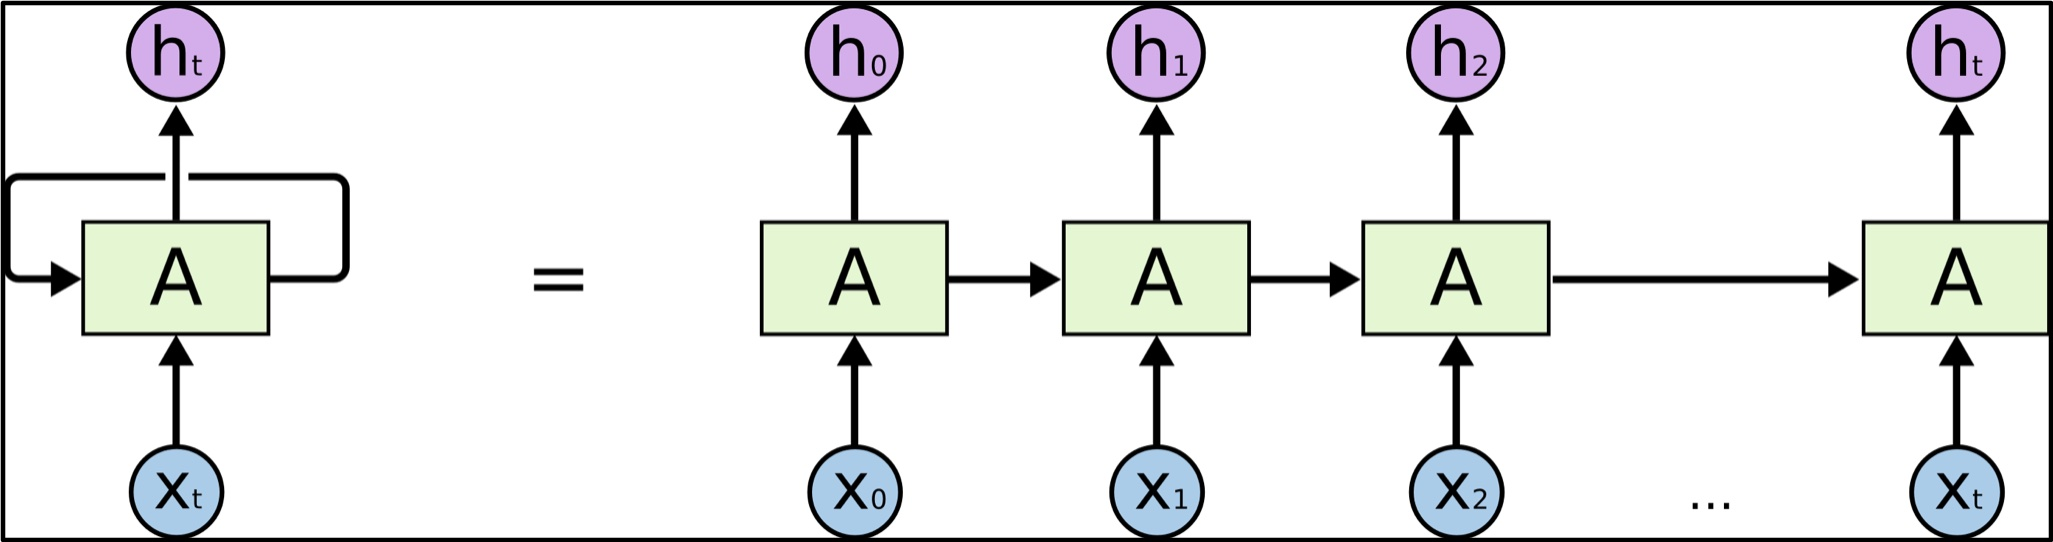
\includegraphics[scale = 0.2]{figures/RNN.jpg}
\end{figure}


where $X_t$ is input data at time $t$, $A$ is Hidden layer, and $h_t$ is an output from RNN at time $t$ shown in Figure \ref{fig:RNN}. The main benefit of this loop is to bring back the previous hidden state, or simply say that RNN is a Neural Network with more memory to store the previously calculated hidden state.


The main problem in RNNs is called the ``vanishing gradient'' problem. To update the weights in a neural networks, we use backpropagation of loss using chain rules for the gradient \cite{arnx_2019}. We calculate the gradient of the loss function ($E$) with respect to the parameters, as shown in Figure \ref{fig:bpp}. RNNs are more complicated, because the output $h_t$ depends not only on timestep $t$, but also on timesteps $t-1, t-2, ..., 1$. Therefore, the backpropagation has to include all calculations from the first timestep to the last. When the gradient magnitude is less than one, a series continuous multiplications will cause the gradient magnitude to decrease as the sequence gets longer. Specifically, the simple RNNs still have difficulties with data with sequential dependencies over a long period of time.

\begin{figure}[H]
  \centering
  \caption[The concept of optimization in a feed-forward neural network.]{\emph{The concept of optimization in a feed-forward neural network. \\Reprinted from \citeauthor{donges_2019}. \citeyear{donges_2019}}}\label{fig:bpp}
  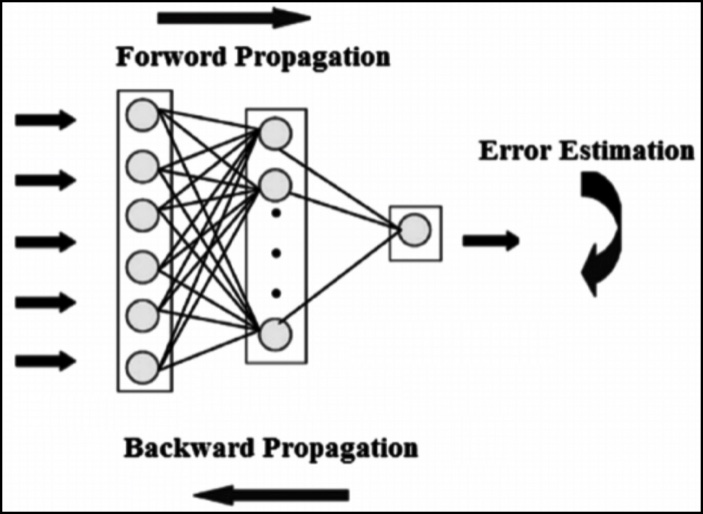
\includegraphics[scale = 0.4]{figures/bpp.jpg}
\end{figure}

\begin{figure}[H]
  \centering
  \caption[The repeating module in a standard RNN contains a single layer.]{\emph{The repeating module in a standard RNN contains a single layer. \\Reprinted from \citeauthor{olah_2015} \citeyear{olah_2015}.}}\label{fig:RNN_2}
  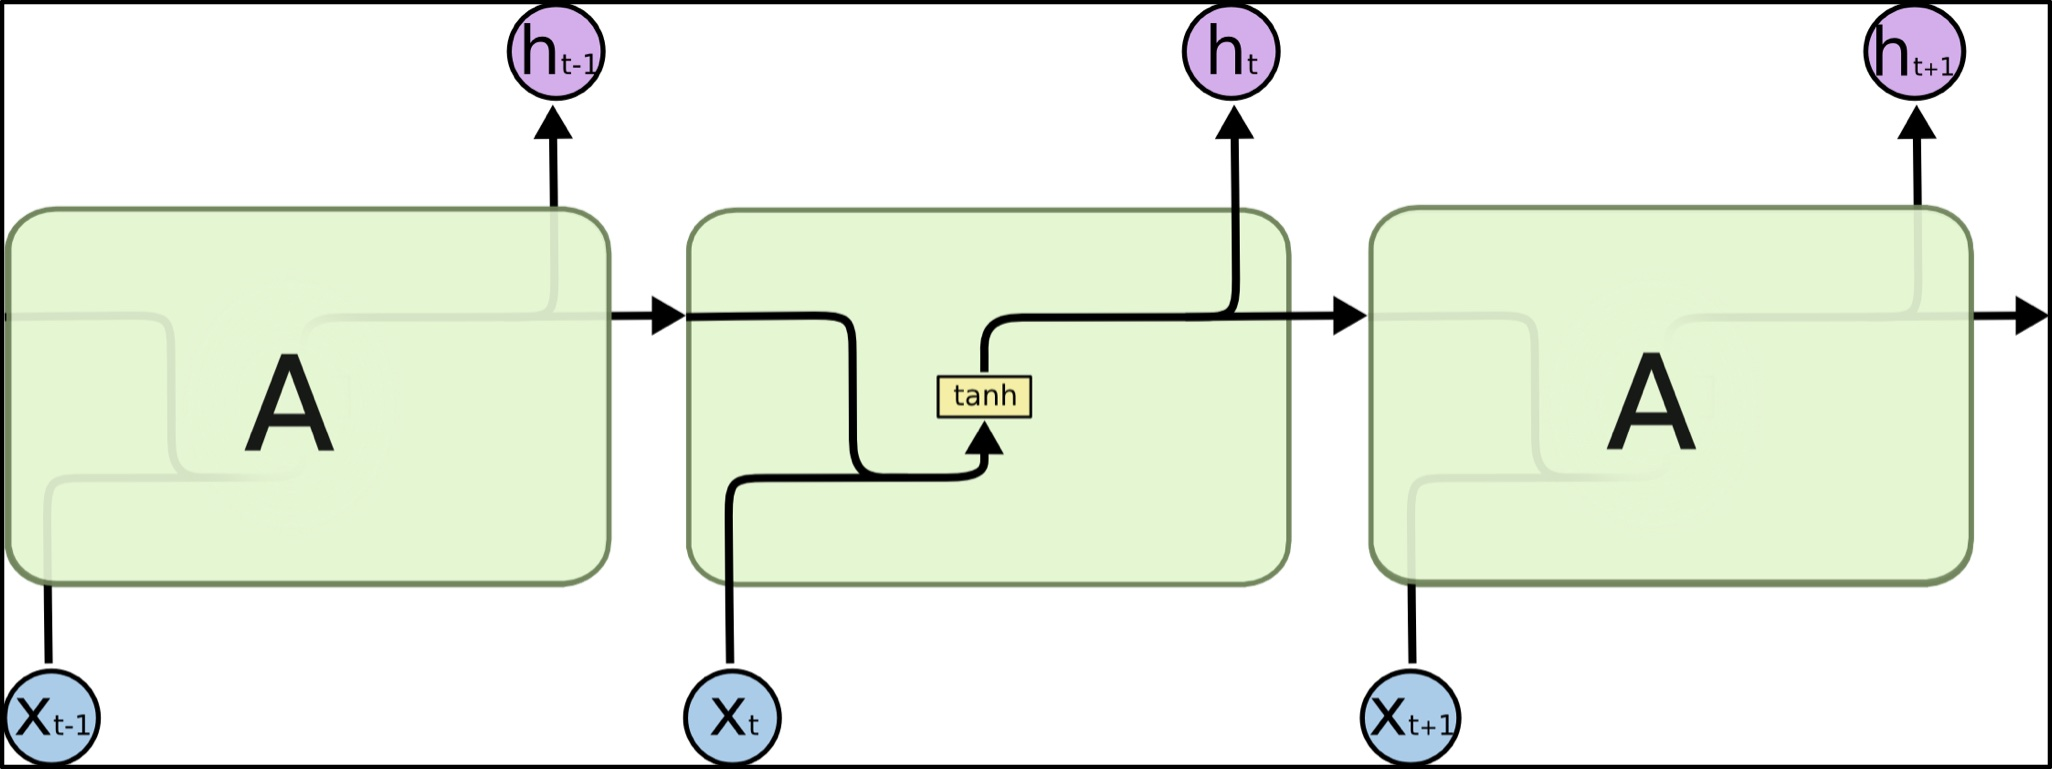
\includegraphics[scale = 0.2]{figures/RNN_2.jpg}
\end{figure}

\section{Long Short-Term Memory (LSTM)}

Long short-term memory networks are an extension of simple RNNs that attempt to mitigate the problem of vanishing gradient under long term dependencies. LSTMs are well suited to learn from important events with long time lags in between \cite{donges_2019,olah_2015}. This is accomplished by giving the memory (hidden state) gates enabling forget (delete), write, and read, as shown in Figure \ref{fig:LSTM}.

\begin{figure}[H]
  \centering
  \caption[LSTM structure.]{\emph{LSTM structure. \\ Reprinted from  \citeauthor{sirinart_tangruamsub_2017} \citeyear{sirinart_tangruamsub_2017}.}}\label{fig:LSTM}
  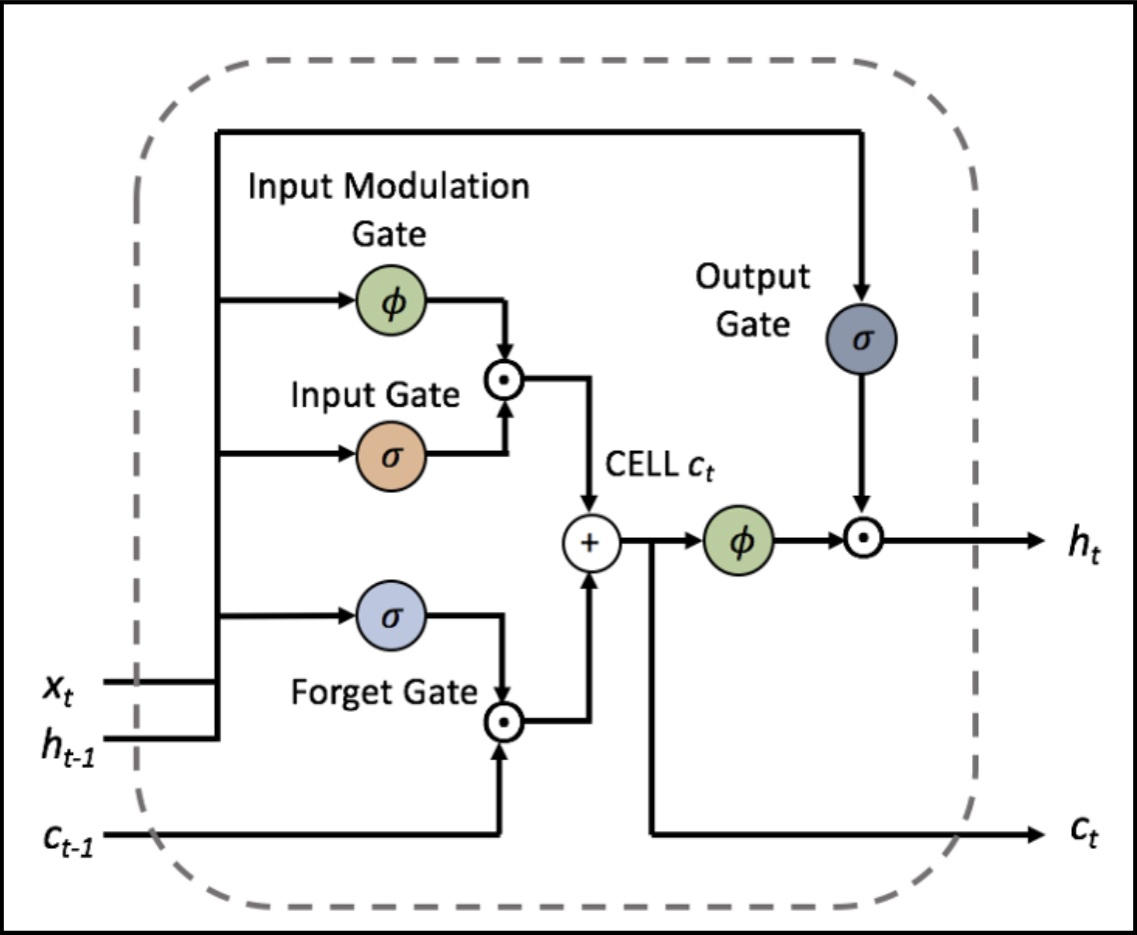
\includegraphics[scale = 0.3]{figures/LSTM.jpg}
\end{figure}


Before specifying the LSTM's details, some variables are needed \cite{sirinart_tangruamsub_2017}:
\begin{itemize}
  \item Cell state: The LSTM's memory.
  \item Gate: A module controling the flow of data, e.g., allowing a write, a read, or a forget operation.
\end{itemize}

The three operations in a LSTM are as follows.


\textbf{Forget}: Forgeting involves (partly or wholly) clearing an old cell state in preparation for new input. The forget gate has the responsibility of deciding whether to clear cell state. If the forget gate outputs zero, the previous cell state is cleared completely. If the forget gate outputs a one, the model retains the cell state completely. In between 0 and 1, the state is attenuated proportionally. The forget gate integrates the incoming input data and the previous hidden state (according to the RNN formula) for making decisions. A sigmoid activation is to limit the gate range to 0 - 1. The gate output $f_t$ is defined as

\hfil $ f_t = \sigma(\mathbf{W_{x^f}}x_t + \mathbf{W_{h^f}}h_{t-1} + b_f) $, \par

where $\mathbf{W_{x^f}}$ is the linear weight vector applied to the model's input at time $t$, $\mathbf{W_{h^f}}$ is the linear weight vector for the hidden state propagated from time $t-1$, $x_t$ is the incomming input, $h_{t-1}$ is the previous hidden state, $b_f$ is the forget gate bias, and $\sigma$ is the sigmoid function.


\textbf{Write}: When new input is fed to the model, it first must decide whether to update its cell state. This action is controlled by an input gate also using a sigmoid activation. This computation is

\hfil $ i_t = \sigma(\mathbf{W_{x^i}}x_t + \mathbf{W_{h^i}}h_{t-1} + b_i) $, \par

where $i_t$ is output of the input gate, $\mathbf{W_{x^i}}$ is the linear weight vector for the input, $\mathbf{W_{h^i}}$ is the weight vector for the hidden state, $x_t$ is the input, $h_{t-1}$ is the previous hidden state, $b_i$ is the input gate bias, and $\sigma$ is the sigmoid function. Secondly, if the model decides to do an update ($i_t$ is large), what value should it update with? This question is answered by the “Input modulation gate”. The input modulation gate uses a tanh function instead of a sigmoid. The gate value is

\hfil $ g_t = \tanh(\mathbf{W_{x^c}}x_t + \mathbf{W_{h^c}}h_{t-1} + b_c) $, \par

where $g_t$ is the input modulation gate's output, $\mathbf{W_{x^c}}$ is the linear weight vector for the input, $\mathbf{W_{h^c}}$ is the linear weight vector for the hidden state, $x_t$ is the input, $h_{t-1}$ is the previous hidden state, $b_c$ is the input modulation gate bias, and $\tanh$ is the hyperbolic tangent function.


\textbf{Update cell state}: Once the forget gate, input gate, and input modulation gate values are calculated, the cell state is updated as

\hfil $c_t = f_t \circ c_{t-1} + i_t \circ g_t $, \par

where $c_t$ is the current cell state and $c_{t-1}$ is the previous cell state. Clearly, the forget gate optionally deletes the old cell state when $f_t$ is zero. When $f_t$ is a one, the model can propagates $c_{t -1}$. When $i_t$ is a one, the input modulation gate $g_t$ provides the update, based on the current input and previous hidden state. If $i_t$ is close to zero, $g_t$ is overlooked.


\textbf{Read}: In sample RNNs, the model produces a hidden state $h_t$ on each time $t$. At  time $t+1$, a LSTM similarly takes the previous $h_t$. The term “read” for a LSTM means to allow a downstream elements to read $h_t$ or to block the $h_t$ value from being propagated. The output gate is calculated by

\hfil $ o_t = \sigma(\mathbf{W_{x^o}}x_t + \mathbf{W_{h^o}}h_{t-1} + b_o) $, \par

where $\mathbf{W_{x^o}}$ is the linear weight vector of the input, $\mathbf{W_{h^o}}$ is the linear weight vector of the hidden state, $x_t$ is the input, $h_{t-1}$ is the previous hidden state, and $b_o$ is the output gate bias. The output $o_t$ is propagated to the next timestep in order to control read operation, i.e.,

\hfil $ h_t = o_t \circ \tanh(c_t) $. \par
If the output gate $o_t$ is zero, $h_t$ is attenuated to zero meaning nothing is sent. On the other hand, if $o_t$ is one, the model propagates $h_t$ as an output and propagates.

\begin{figure}[H]
  \centering
  \caption[The repeating module in a LSTM contains four interacting layer.]{\emph{The repeating module in a LSTM contains four interacting layer. \\Reprinted from \citeauthor{olah_2015} \citeyear{olah_2015}.}}\label{fig:LSTM_2}
  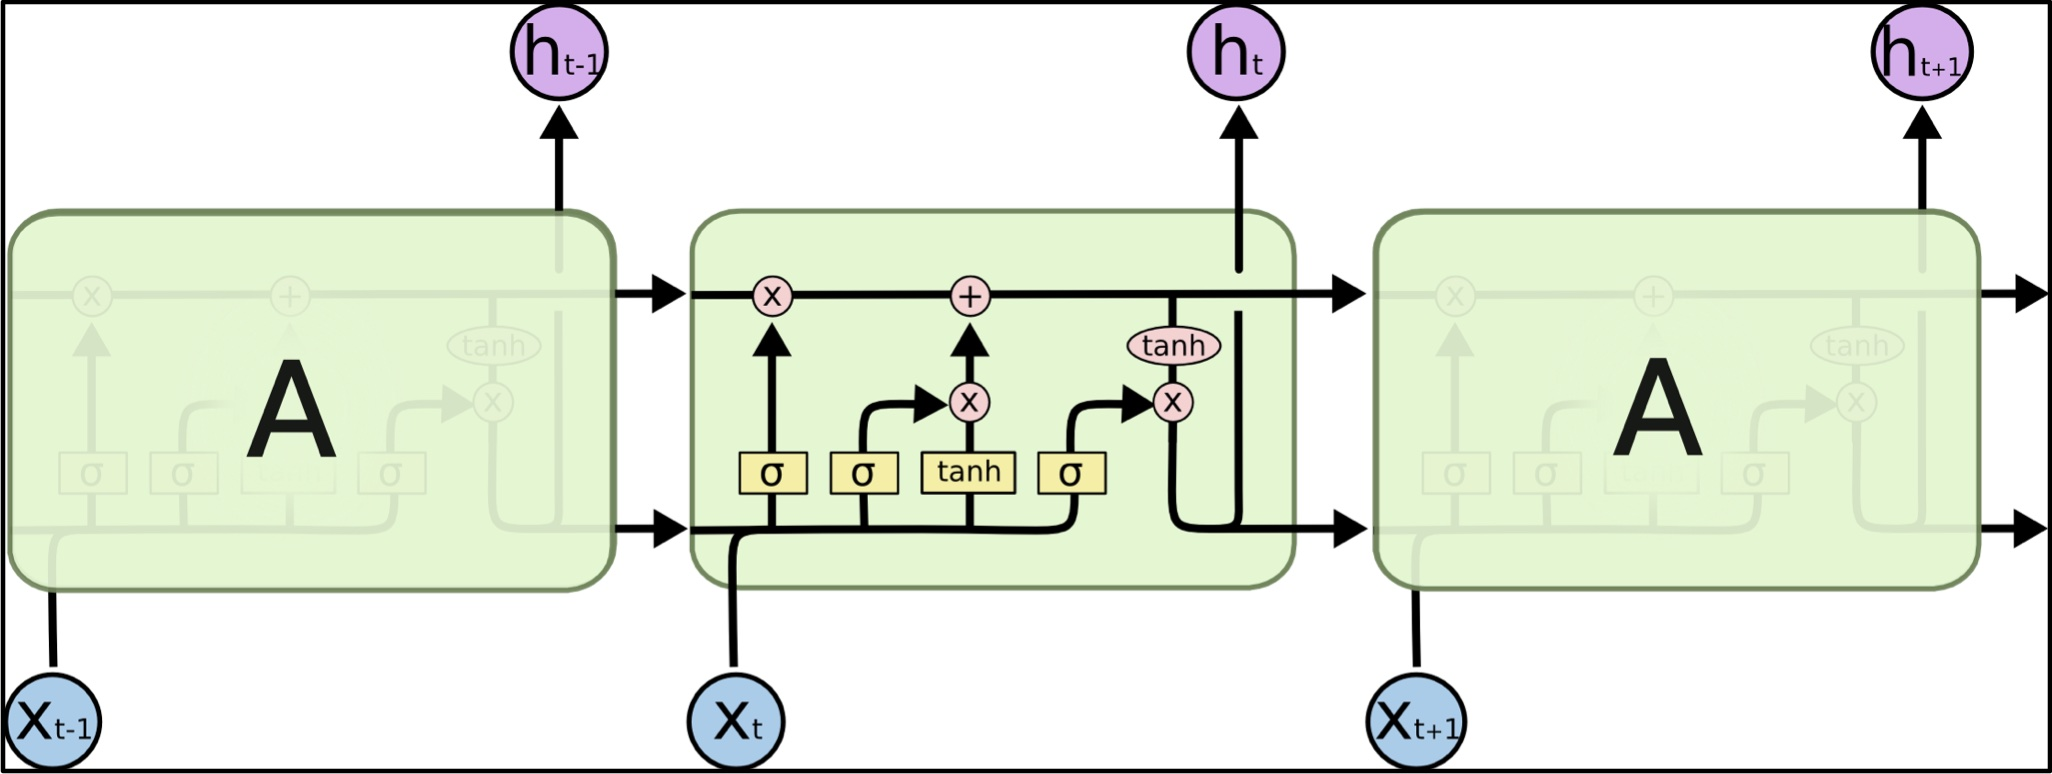
\includegraphics[scale = 0.14]{figures/LSTM_2.jpg}

\end{figure}

\section{Transformer}

The transformer was proposed in the paper ``Attention is All You Need'' by Google \cite{vaswani_shazeer_parmar_uszkoreit_jones_n_gomez_kaiser_polosukhin_2017}. This paper proposes a new architecture that replaces RNNs time-locked processing with an attention mechanism called the transformer, as shown in Figure \ref{fig:attention}. The transformer architecture has recently beat benchmarks in many domains. In particular, it has revolutionized the Natural Language Processing (NLP) field, particularly in the machine translation task. This model contains two significant parts, an encoder and a decoder, which work as similar as an autoencoder. In principle, transformers can be used for anomaly detection purposes as well \cite{mishra_verk_fornasier_piciarelli_foresti_2021}.

\begin{figure}[H]
  \centering
  \caption[The transformer architecture.]{\emph{The transformer architecture. \\Reprinted from \citeauthor{vaswani_shazeer_parmar_uszkoreit_jones_n_gomez_kaiser_polosukhin_2017} \citeyear{vaswani_shazeer_parmar_uszkoreit_jones_n_gomez_kaiser_polosukhin_2017}.}}\label{fig:attention}
  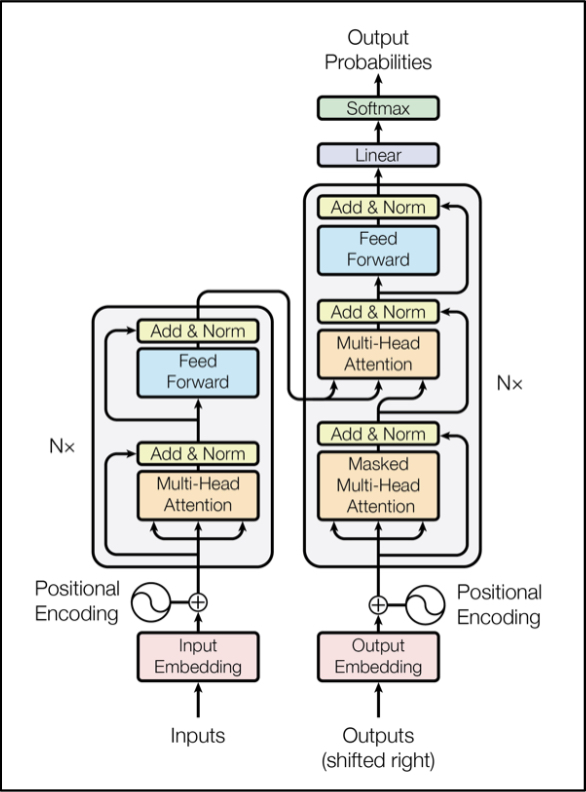
\includegraphics[scale = 0.4
  ]{figures/attention.jpg}
\end{figure}


To compare how RNNs and attention deals with the time dimension of the input, RNNs include every information needed about sequential data into the final hidden state of the network. The decision layer can only access the memory accumulated at that timestep. At every timestep, the RNN focuses on a different positions in the input. On the other hand, an attention mechanism can focus on any of the input from several timesteps, and setting weights on each input indicating what should be focused on in order to make a prediction. Figure \ref{fig:rnnvsattention} provides the intuition behind both methods.

\begin{figure}[H]
  \centering
  \caption[Comparison RNNs and Attention.]{\emph{Comparison RNNs and Attention.}}\label{fig:rnnvsattention}
  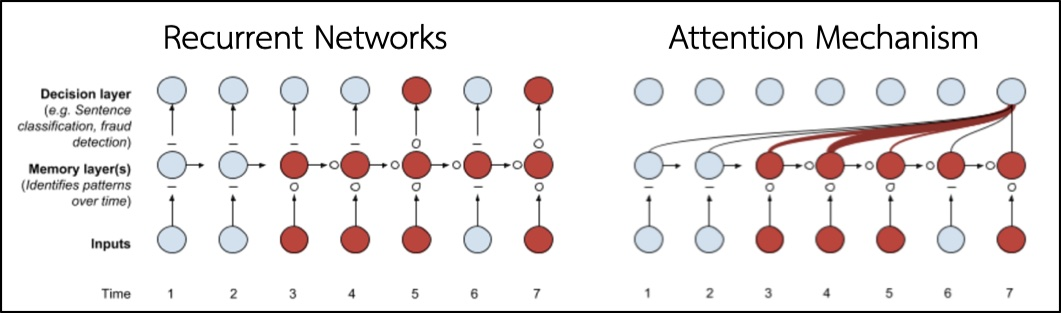
\includegraphics[scale = 0.4
  ]{figures/rnnvsattention.jpg}
\end{figure}
\subsection{Attention}

According to \citeauthor{james_1890} \citeyear{james_1890}, in psychology, attention is a concentration of the mind on a single object or thought, one preferentially selected from among many stimuli using possibly complex process, with a view to limiting or clarifying receptivity by narrowing the range of stimuli. Similarly, attention in neural networks was specifically designed to focus on only the most important subsets of long sequences related to completing a given task \cite{alammar_2018,alammar_2019,klingenbrunn_2021}. The process consists of three main steps, as follows.
\begin{enumerate}
  \item Create the query (representing the current position vector in the input sequence), key (representing the relative importance of the inputs in the sequence), and value (representing the priority of each position) vectors, they are quite useful for calculating and thinking about attention, for each path and each input token by multiplying by weight matrices as $W^Q$, $W^K$ and $W^V$ as shown in Figure \ref{fig:attention_2}.
  \item For each input token, use the query vector to get a score against all the other key vectors by multiplying the current query vector with all the key vectors as shown in Figure \ref{fig:attention_3}.
  \item Sum up the value vectors after multiplying them by their associated scores. More transparent blocks in Figure \ref{fig:attention_4} are those with lower values.

\end{enumerate}


If the model performs the same operation for each input token, the result is a vector representing the context of each token, as shown in Figure \ref{fig:attention_5}. These vectors are passed to the next sub layer in the transformer block.

\begin{figure}[H]
  \centering
  \caption[Creating the query, key and value vector in a self-attention module.]{\emph{Creating the query, key and value vector in a self-attention module. \\
      Reprinted from \citeauthor{alammar_2018} \citeyear{alammar_2018}.}}\label{fig:attention_2}
  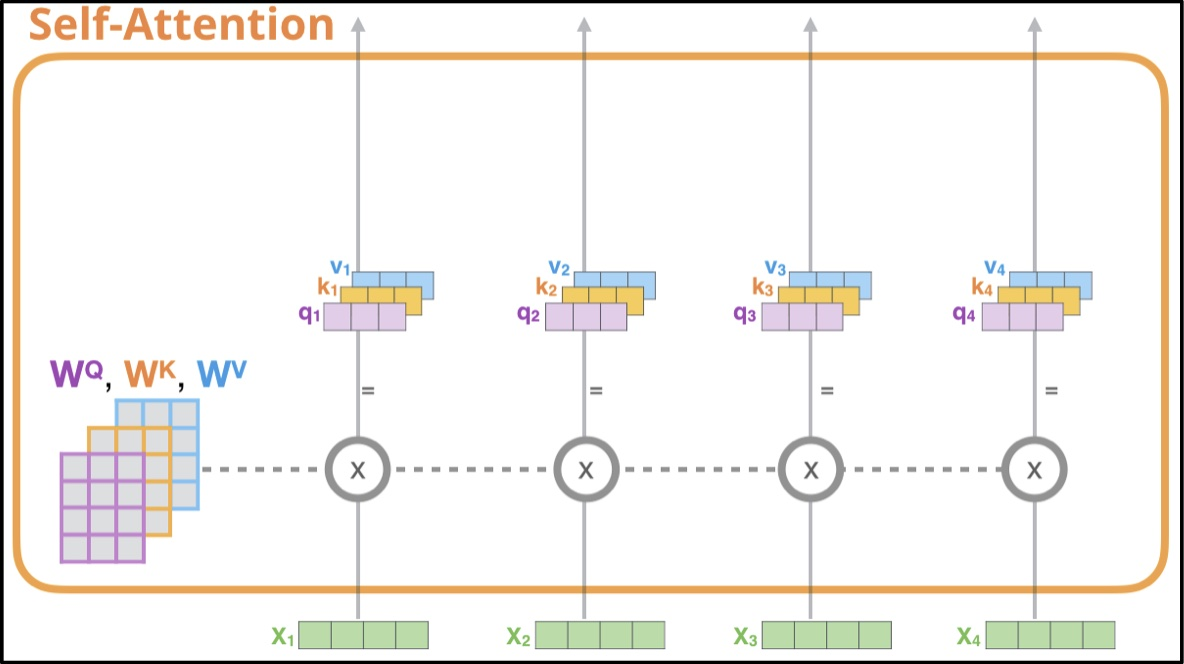
\includegraphics[scale = 0.3]{figures/attention_2.jpg}
\end{figure}

\begin{figure}[H]
  \centering
  \caption[Getting a score of how each key matches the query in a self-attention module.]{\emph{Getting a score of how each key matches the query in a self-attention module. \\
      Reprinted from \citeauthor{alammar_2018} \citeyear{alammar_2018}.}}\label{fig:attention_3}
  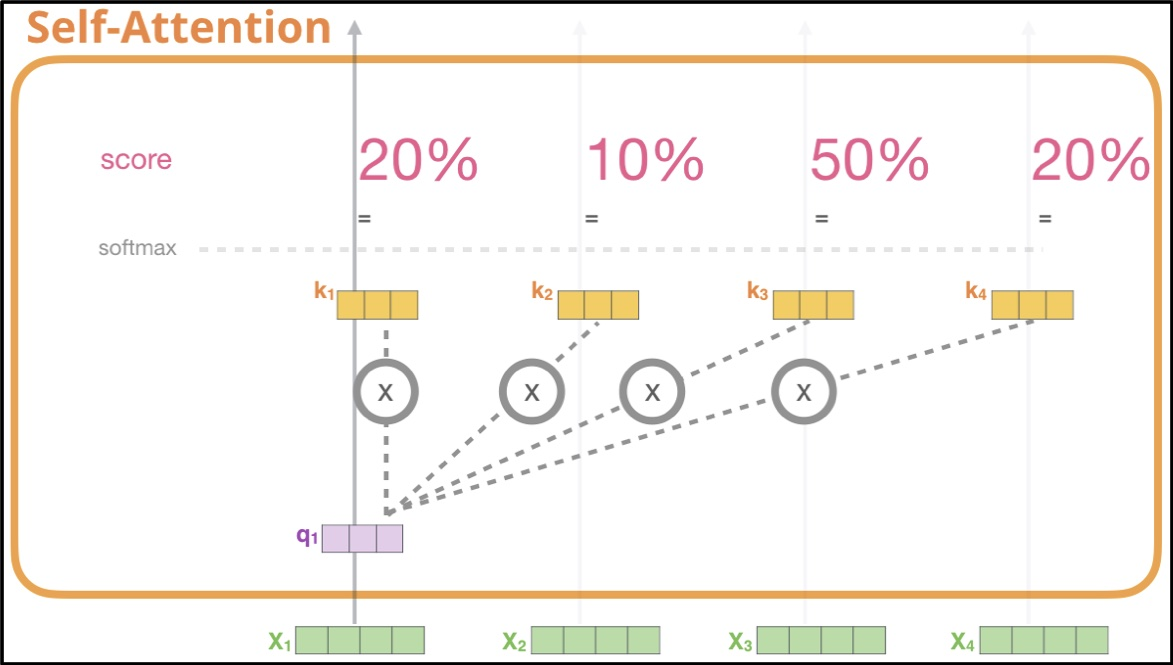
\includegraphics[scale = 0.3]{figures/attention_3.jpg}
\end{figure}

\begin{figure}[H]
  \centering
  \caption[Summing up the value vectors in a self-attention module.]{\emph{Summing up the value vectors in a self-attention module. \\
      Reprinted from \citeauthor{alammar_2018} \citeyear{alammar_2018}.}}\label{fig:attention_4}
  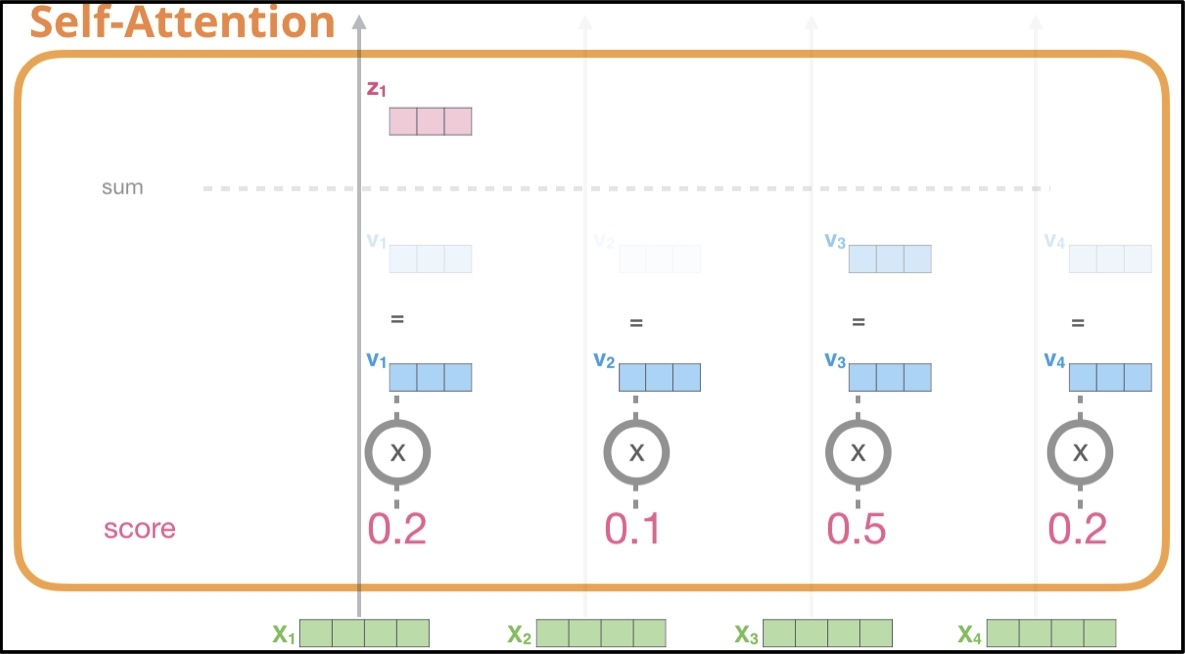
\includegraphics[scale = 0.3]{figures/attention_4.jpg}
\end{figure}
\begin{figure}[H]
  \centering
  \caption[The outcome of the self-attention process.]{\emph{The outcome of the self-ttention process. \\Reprinted from \citeauthor{alammar_2018} \citeyear{alammar_2018}.}}\label{fig:attention_5}
  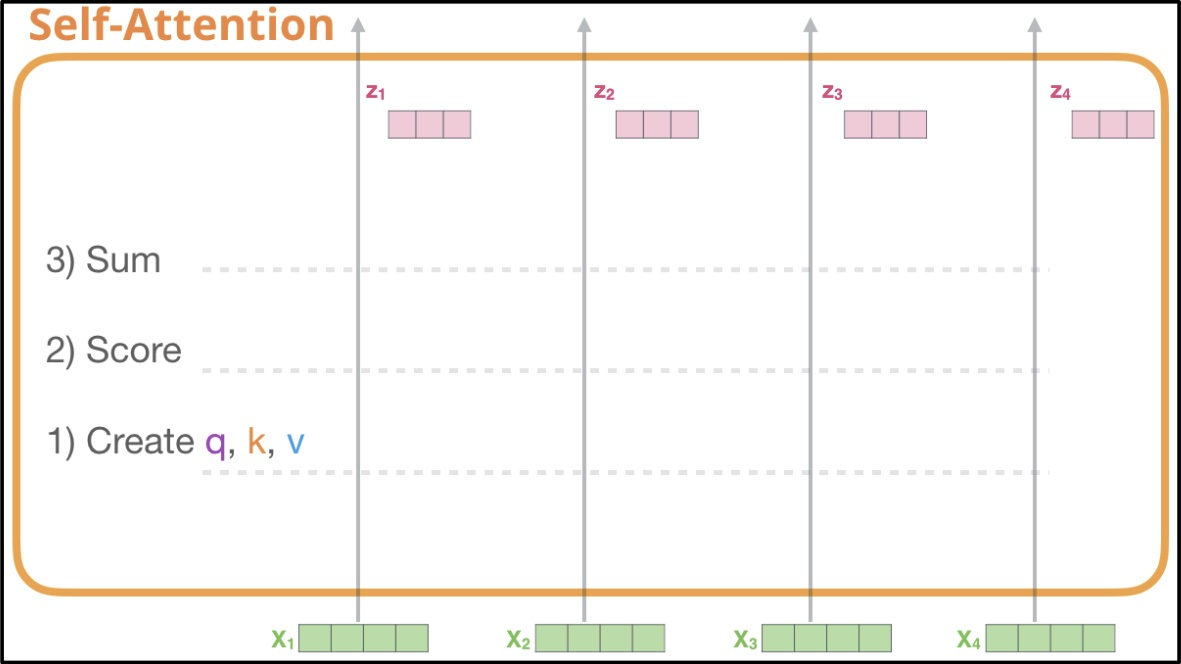
\includegraphics[scale = 0.3]{figures/attention_5.jpg}
\end{figure}


Note that in the decoder, a transformer uses masked self-attention. The difference between self-attention and masked self-attention is shown Figure \ref{fig:attention_6}. A self-attention allows each position in the output to attend to all positions in the input but Masked Self-Attention only considers previous positions in order to preserve the auto-regressive property.

\begin{figure}[H]
  \centering
  \caption[Difference between self-attention and masked self-attention.]{\emph{Difference between self-attention and masked self-attention. \\ Reprinted from \citeauthor{alammar_2019} \citeyear{alammar_2019}.}}\label{fig:attention_6}
  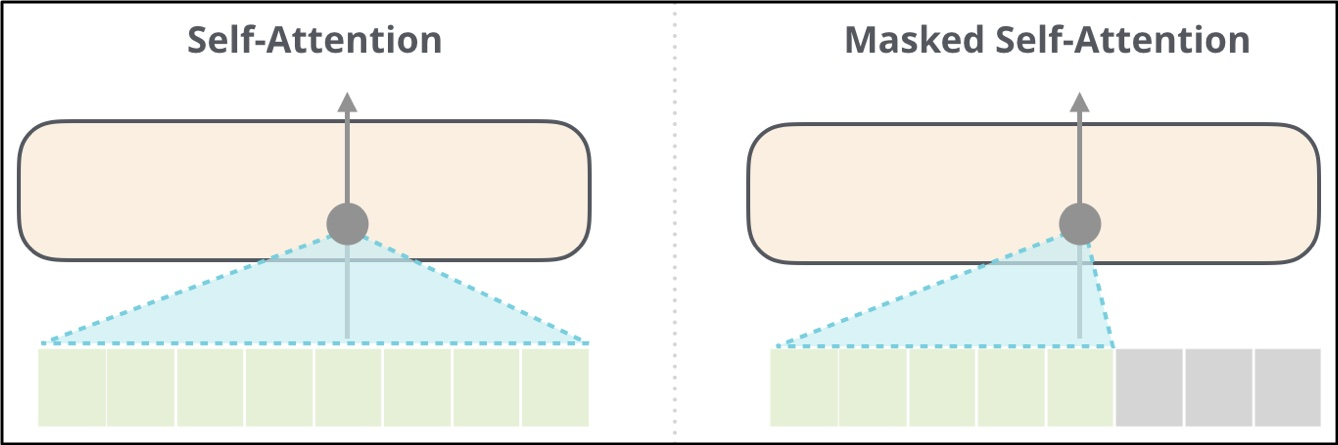
\includegraphics[scale = 0.3]{figures/attention_6.jpg}
\end{figure}
\subsection{Positional Encoding}


In any sequence to sequence model in which the number of inputs or outputs is variable and order and position are important, if we are not using recurrence or convolution, we need some other principle to make use of the order an input sequence, as shown in Figure \ref{fig:attention_7}. The formulae for positional encoding are

\hfil $PE(pos, 2i) = \sin(\frac{pos}{10000^{2i/d_{model}}})$, \par
\hfil $PE(pos, 2i + 1) = \cos(\frac{pos}{10000^{2i/d_{model}}})$, \par

where $pos$ is the index of a token $\in[0, L-1]$ in the input sequence, $d_{model}$ is the model depth, and $i$ is an along the model depth. The important characteristics of positional encoding are

\begin{enumerate}
  \item Positional encoding is represent by a matrix with dimension (sequence length $\times$ model depth).
  \item Each column of the PE matrix represents the continuous value which varies according to the $pos$ value.
  \item Each row of the PE matrix represents the interpolated position of the discrete value.
  \item The row vectors are alternating series of sines and cosines, with frequencies that decrease according to a geometric series.
\end{enumerate}

\begin{figure}[H]
  \centering
  \caption[Positional encoding of a sequence length of length 50 in a model with a model depth of 256.]{\emph{Positional encoding of a sequence length of length 50 in a model with a model depth of 256. \\ Reprinted from \citeauthor{tamura_2021} \citeyear{tamura_2021}.}}\label{fig:attention_7}
  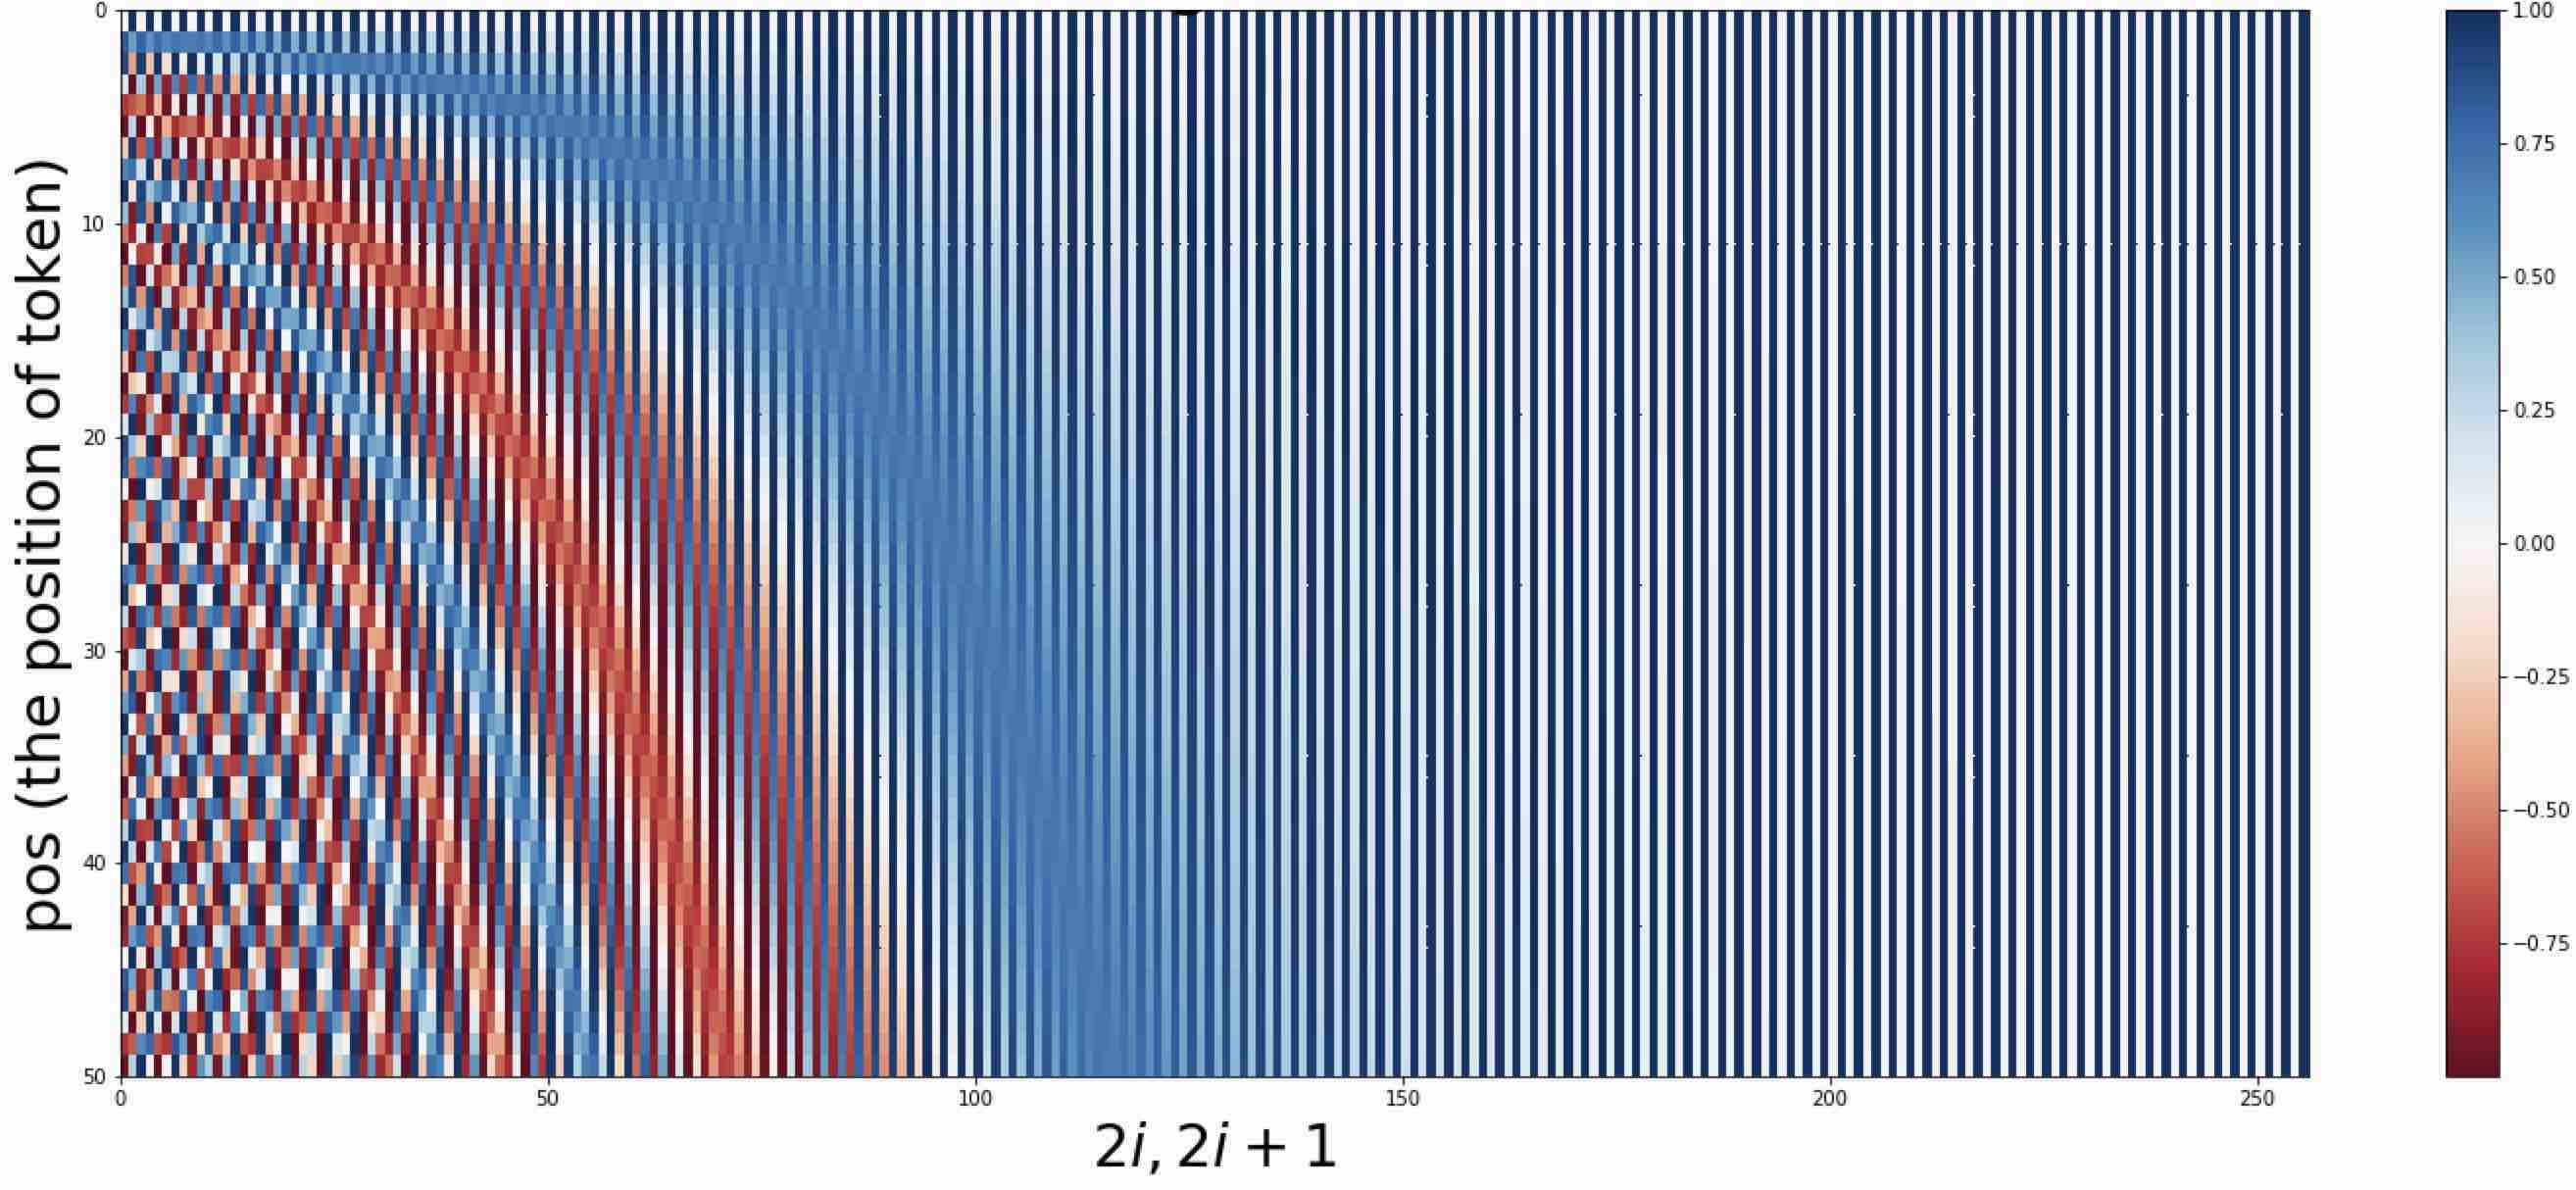
\includegraphics[scale = 0.15]{figures/positional_encoding.jpg}
\end{figure}

\section{Notch filter}

A notch filter is a type of band-stop filter that attenuates frequencies within a certain range while passing all other frequencies unchanged. The attenuated frequency range is extremely small (high Q factor). A nothch filter is the opposite of a band-pass filter. Notch filters are important when we need to reject noise or other artifacts occurring at specific frequencies with a narrow bandwidth. Figure \ref{fig:notch} illustrates the magnitude and phase of a notch filter set to attenuate frequencies around 10 Hz.

\begin{figure}[H]
  \centering
  \caption[Bode diagram of notch filter]{\emph{Bode diagram of notch filter \\ Reprinted from Google.}}\label{fig:notch}
  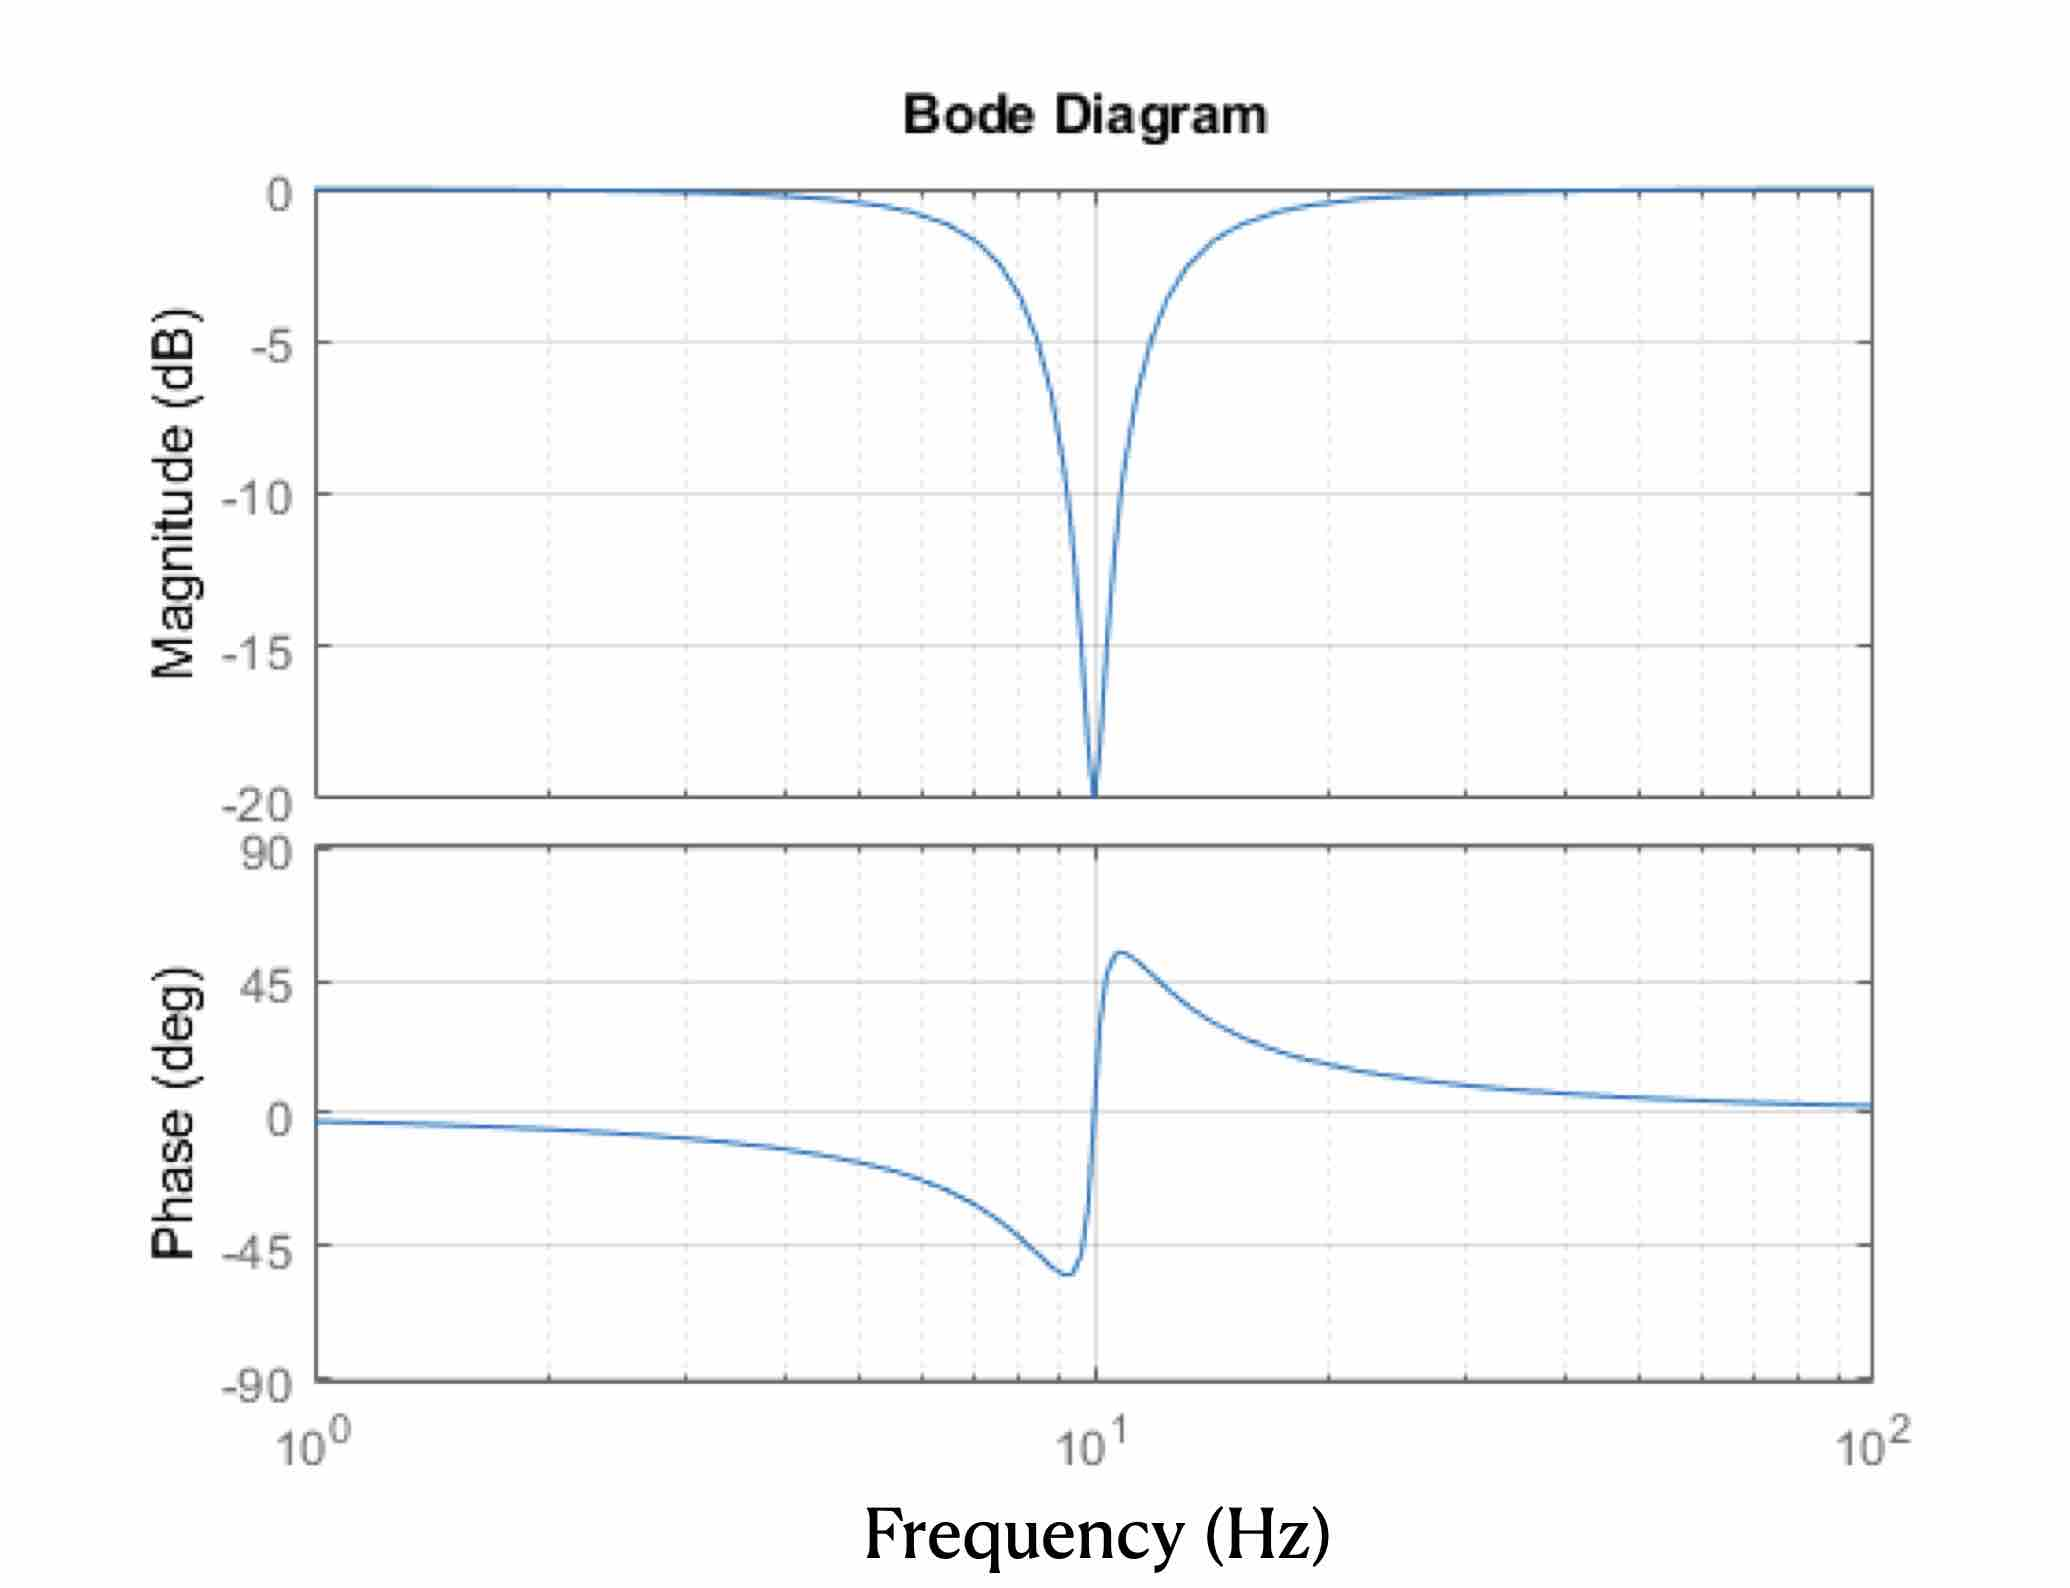
\includegraphics[scale = 0.2]{figures/notch.jpg}
\end{figure}

\section{Principal components analysis}
Principal components analysis or PCA is the dimensionality reduction algorithm which belong to unsupervised learning. Eventhough this algorithm was invented in 1901, it is still one of the most normally used technique for reduce dimension. Basically, reduction dimensions of a original can lead to reduce an accuracy \cite{patel_2019}. However, the benefit of reducing dimension is to trade of between a few accuracy and simplicity. PCA is an orthogonal linear transformation by create vectors to representation original data and then transforms these data to the new coordinate system \cite{vanderplas_2017} as shown in Figure \ref{fig:pca}

\begin{figure}[H]
  \centering
  \caption[The input and output of PCA.]{\emph{The input and output of PCA. \\ Reprinted from \citeauthor{vanderplas_2017} \citeyear{vanderplas_2017}.}}\label{fig:pca}
  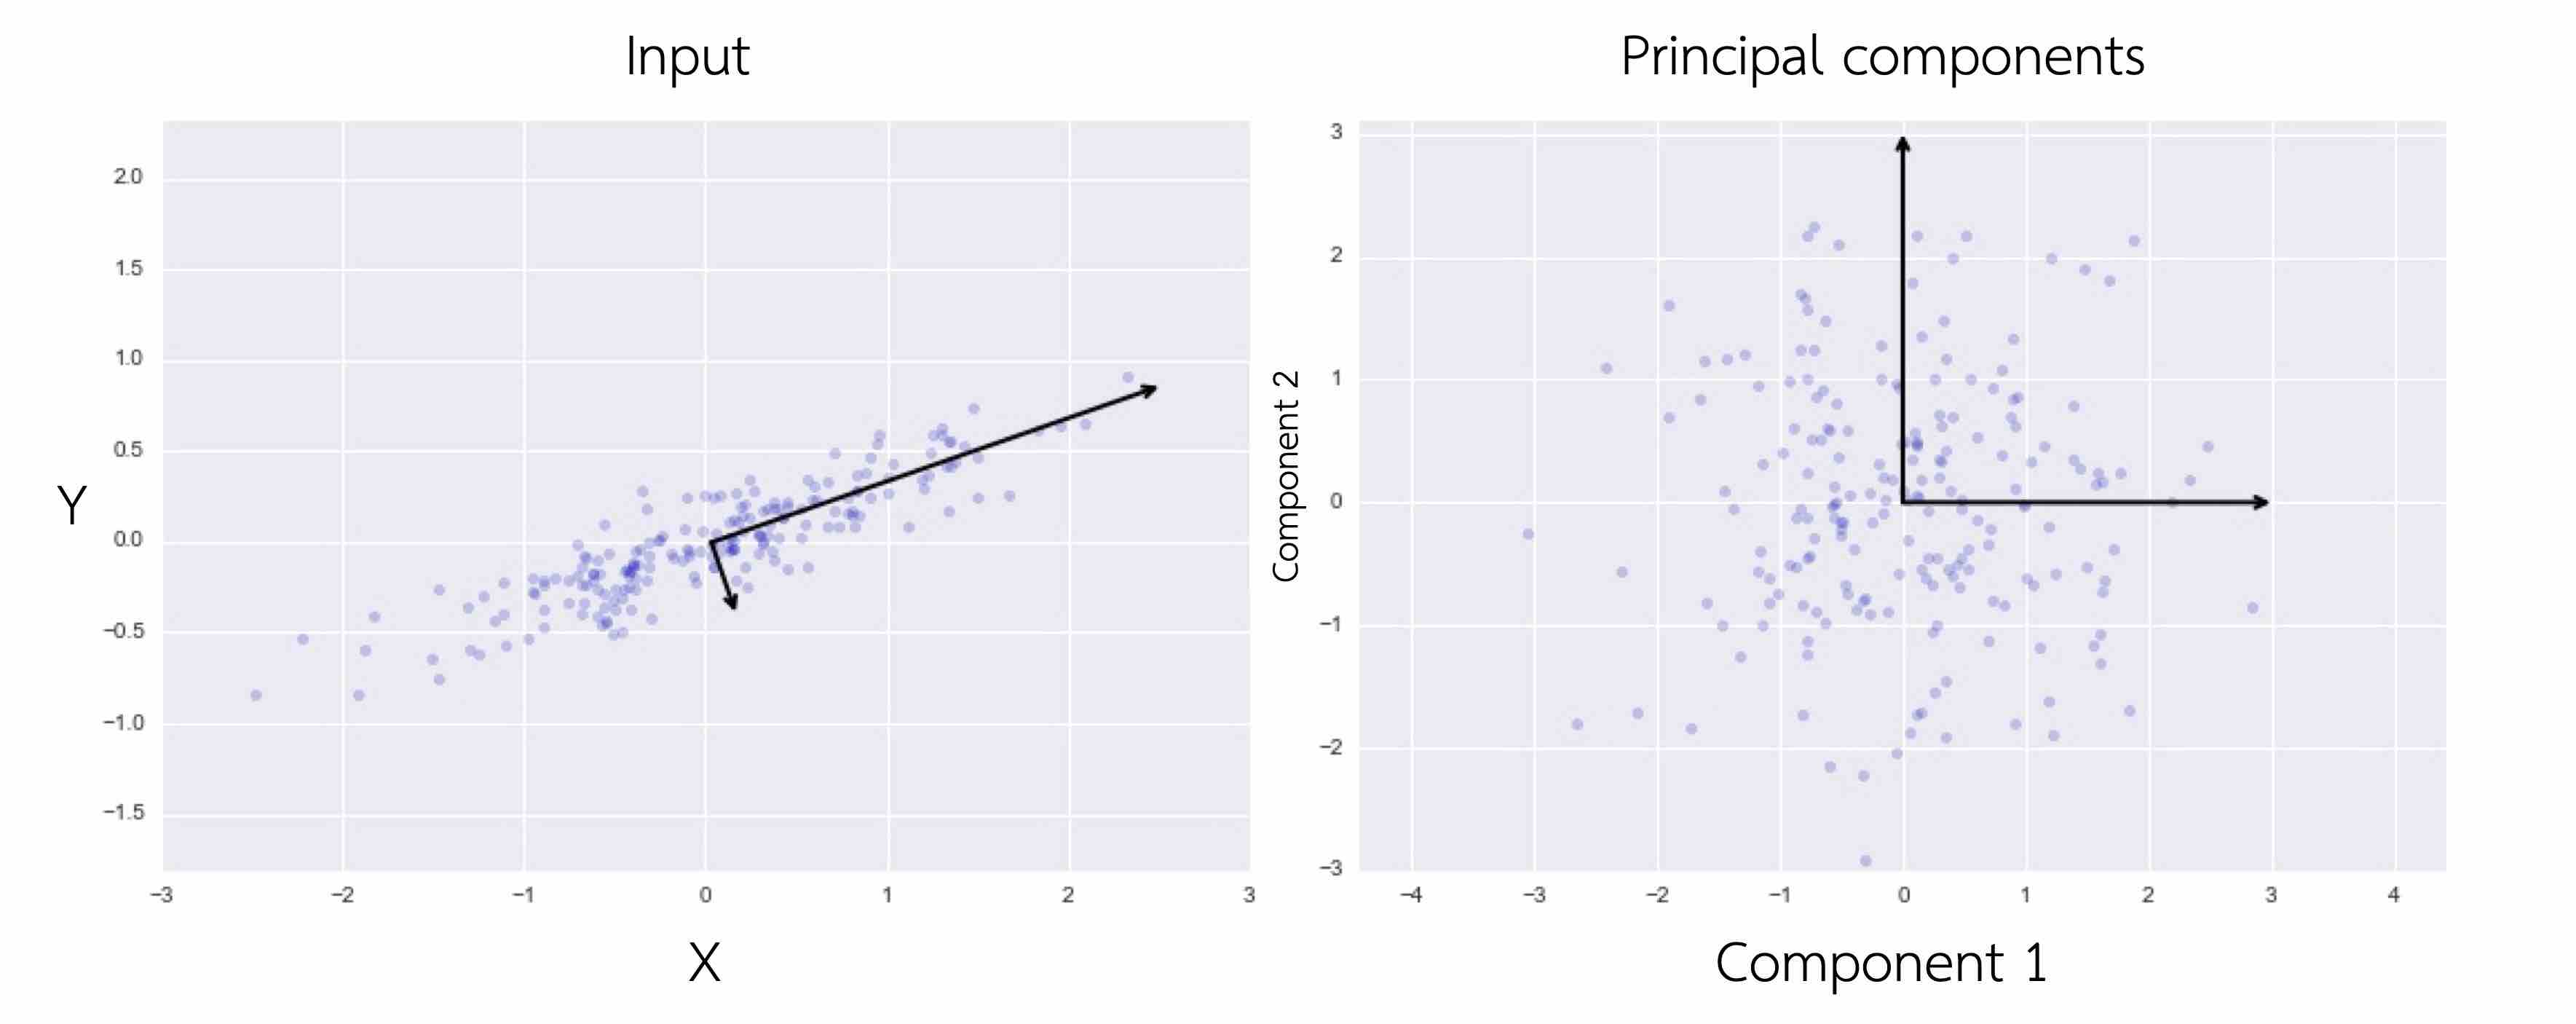
\includegraphics[scale = 0.13]{figures/pca.jpg}
\end{figure}

\FloatBarrier